%%%%%%%%%%%%%%%%%%%%%%%%%%%%%%%%%%%%%%%%%%%%%%%%%%%%%%%%%%%%%%%%%%%%%%
% amspaper.tex --  LaTeX-based template for submissions to American 
% Meteorological Society journals
%
% Template developed by Amy Hendrickson, 2013, TeXnology Inc., 
% amyh@texnology.com, http://www.texnology.com
% following earlier work by Brian Papa, American Meteorological Society
%
% Email questions to latex@ametsoc.org.
%
%%%%%%%%%%%%%%%%%%%%%%%%%%%%%%%%%%%%%%%%%%%%%%%%%%%%%%%%%%%%%%%%%%%%%
% PREAMBLE
%%%%%%%%%%%%%%%%%%%%%%%%%%%%%%%%%%%%%%%%%%%%%%%%%%%%%%%%%%%%%%%%%%%%%

%% Start with one of the following:
% DOUBLE-SPACED VERSION FOR SUBMISSION TO THE AMS
\documentclass{ametsoc}

% TWO-COLUMN JOURNAL PAGE LAYOUT---FOR AUTHOR USE ONLY
% \documentclass[twocol]{ametsoc}

%%%%%%%%%%%%%%%%%%%%%%%%%%%%%%%%
%%% To be entered only if twocol option is used

\journal{jcli}

\usepackage{color}

%  Please choose a journal abbreviation to use above from the following list:
% 
%   jamc     (Journal of Applied Meteorology and Climatology)
%   jtech     (Journal of Atmospheric and Oceanic Technology)
%   jhm      (Journal of Hydrometeorology)
%   jpo     (Journal of Physical Oceanography)
%   jas      (Journal of Atmospheric Sciences)	
%   jcli      (Journal of Climate)
%   mwr      (Monthly Weather Review)
%   wcas      (Weather, Climate, and Society)
%   waf       (Weather and Forecasting)
%   bams (Bulletin of the American Meteorological Society)
%   ei    (Earth Interactions)

%%%%%%%%%%%%%%%%%%%%%%%%%%%%%%%%
%Citations should be of the form ``author year''  not ``author, year''
\bibpunct{(}{)}{;}{a}{}{,}

%%%%%%%%%%%%%%%%%%%%%%%%%%%%%%%%

%%% To be entered by author:

%% May use \\ to break lines in title:

\title{The changing character of twenty-first century precipitation over the western United States in the variable-resolution CESM}


%Future changes of precipitation over Western United States using variable-resolution CESM 

%change the title?

%%% Enter authors' names, as you see in this example:
%%% Use \correspondingauthor{} and \thanks{Current Affiliation:...}
%%% immediately following the appropriate author.
%%%
%%% Note that the \correspondingauthor{} command is NECESSARY.
%%% The \thanks{} commands are OPTIONAL.

    \authors{Xingying Huang, \correspondingauthor{Xingying Huang, 
     Department of Land, Air and Water Resources,
     University of California Davis, Davis, CA 95616.}
     Paul A. Ullrich}

     \affiliation{Department of Land, Air and Water Resources, University of California, Davis}

\email{xyhuang@ucdavis.edu}


    \extraauthor{}
    \extraaffil{}


%%%%%%%%%%%%%%%%%%%%%%%%%%%%%%%%%%%%%%%%%%%%%%%%%%%%%%%%%%%%%%%%%%%%%
% ABSTRACT
%
% Enter your Abstract here

\abstract{({\color{red} To be added once the main content settled down})} 

\begin{document}


%% Necessary!
\maketitle


%%%%%%%%%%%%%%%%%%%%%%%%%%%%%%%%%%%%%%%%%%%%%%%%%%%%%%%%%%%%%%%%%%%%%
% MAIN BODY OF PAPER
%%%%%%%%%%%%%%%%%%%%%%%%%%%%%%%%%%%%%%%%%%%%%%%%%%%%%%%%%%%%%%%%%%%%%
%
\section{Introduction}

There is substantial and growing interest in understanding the character of precipitation within a changing climate, in large part because of the pronounced impacts of water availability on socioeconomic and natural systems \citep{hegerl2004detectability, kharin2007changes, scoccimarro2013heavy}.  Among these studies, precipitation extremes have been a major focus, particularly drought and flood events \citep{seneviratne2012changes}. Studies examining the character of precipitation in a warming world, which utilize models of varying complexity from simple thermodynamic models through complex coupled climate simulations, suggest that although atmospheric water vapor is increasing, the consequences for precipitation are far more complicated.  Extreme precipitation events are particularly nuanced:  Our best projections suggest that extreme precipitation events will intensify even in regions where mean precipitation decreases \citep{tebaldi2006going, kharin2007changes}.

%Changes in rainfall distributions have attracted much attention because of the particular vulnerability of human activities to hydrological extreme events such as flood-producing rains and droughts. 
%The intensity of extreme precipitation is projected to increase under global warming in many parts of the world, even in the regions where mean precipitation decreases

%Globally, heat extremes have been increasing, with reducing extreme low temperatures


Although future climate projections are subject to large uncertainties, climate models are nonetheless one of the most versatile tools for studying climate variability and extremes events in the future \citep{easterling2000climate}. Global climate models (GCMs) have often been used to investigate changes in the mean, variability and extremes of climate, as forced with predicted greenhouse gas (GHGs) concentrations and aerosol emissions \citep{meehl2006future}. Several past studies have investigated global impacts \citep{seneviratne2012changes}, but studies addressing impacts at local and regional scales are less common.  Although increased GHG concentrations have contributed to the observed intensification of heavy precipitation events over the tropical ocean \citep{allan2008atmospheric} and the majority of Northern Hemisphere overland areas \cite{min2011human}, these impacts are much more poorly understood at regional scales due to variability at finer spatial scales associated with the atmospheric circulation \citep{trenberth2011changes}.  As a consequence of this variability, a confident assessment of changes in regional extremes requires both high spatial resolution and a long integration period.

%. Precipitation extremes, as measured by various metrics, are predicted to change by future warming based on the results of these simulations

Insufficient regional-scale climate information has been a major outstanding problem in climate science, as stakeholders and water managers typically require fine-scale information on climate impacts in order to effectively develop adaptation and mitigation strategies.  In order to reach the scales needed for effective local planning, dynamical downscaling with regional climate models (RCMs) has been typically used to ascertain the frequency, intensity, and duration of extreme events.  By only simulating a limited regional domain, RCMs better capture fine-scale dynamical features under high horizontal resolution \citep{bell2004regional, frei2006future, rauscher2010resolution, wehner2013very}. Higher resolution can also enable more accurate simulation of precipitation extremes, which can be driven by land use, land/water contrast, snow cover, cloudiness and circulation patterns associated with topography \citep{leung2003regional, diffenbaugh2005fine, salathe2008high, wehner2010effect}. \cite{diffenbaugh2005fine} studied both heat events and wet events over the contiguous United States based on RCMs simulation at 25 km horizontal resolution, and demonstrated that fine-scale processes were critical for accurate assessment of local- and regional-scale climate change vulnerability. \cite{leung2003hydroclimate} showed that the higher-resolution RCMs yield more realistic precipitation patterns and produce more frequent heavy precipitation over the western U.S. (WUS), consistent with observations.

%\citep{mass2011extreme} this paper has detailed discussion of precipitation extremes over western US modeled by other studies. (see the last two paragraphs)

%%wehner2013very   Very extreme seasonal precipitation in the NARCCAP ensemble: model performance and projections
%wehner2010effect  The effect of horizontal resolution on simulation of very extreme US precipitation events in a global atmosphere model
%rauscher2010resolution  Resolution effects on regional climate model simulations of seasonal precipitation over Europe

%singh2013precipitation  Precipitation extremes over the continental United States in a transient, high-resolution, ensemble climate model experiment see the plots
%frei2006future   Future change of precipitation extremes in Europe: Intercomparison of scenarios from regional climate models 

%However, it does not mean that higher resolution can always perform better, and this aspect will be investigated in our study through multi-scale simulations including ~10km horizontal resolution.

%"Simulations with global coupled ocean�atmosphere general circulation models (CGCMs) forced with projected greenhouse gas and aerosol emissions are the primary tools for studying possible future changes in climate mean, variability, and extremes. Changes in rainfall distributions have attracted much attention because of the particular vulnerability of human activities to hydrological extreme events such as flood-producing rains and droughts.

%"climate model improvements have resulted in an enhanced ability to simulate many aspects of climate variability and extremes. However, they are still characterized by systematic errors and limitations in accurately simulating regional climate conditions." \citep{easterling2000climate}

Despite their success, RCMs also have known issues associated with inconsistency between the lateral forcing data and the driven RCM, and the menu of physical parameterizations and parameters typically available to RCMs can lead to over-tuning of the model for a particular geographic region or climatological field \citep{mcdonald2003transparent, laprise2008challenging, mesinger2013limited}.  Consequently, there has been growing interest in variable-resolution enabled GCMs (VRGCMs) to improve regional climate simulations. Unlike RCMs, which require GCM data to drive the simulation at lateral boundaries, VRGCMs use a unified model with coarse global resolution and enhanced resolution over a specific study region \citep{staniforth1978variable, fox1997finite}. VRGCMs have demonstrated comparable utility for regional climate studies at a reduced computational cost, particular when compared to uniform-resolution GCMs \citep{fox2006variable, rauscher2013exploring}.

%Contrasted with RCMs, VRGCMs use a single, unified modeling framework rather than two separate models (GCM and RCM) with potentially disparate dynamics and physical parameterizations, avoiding the inconsistencies and lack of two-way interactions between the global and regional scales at the nest boundary of RCMs  

In this paper, we utilize the recently developed variable-resolution option in the Community Earth System Model (VR-CESM).  VR-CESM is based on the CESM (and its predecessor, the Community Climate System Model (CCSM)), a family of models that have been used for decades to study the global climate \citep{neale2010description, hurrell2013community}.  The overall performance of VR-CESM for modeling regional climate in the California and Nevada is detailed in \cite{huang2016evaluation}, where it was argued that VR-CESM has competitive biases in comparison to the Weather Research and Forecasting (WRF) model (a traditional RCM) and the uniform-resolution CESM, when evaluating both against high-quality observations and reanalysis. VR-CESM has been used in a number of studies to capture fine-scale atmospheric processes  \citep{zarzycki2014using, zarzycki2015effects, rhoades2015characterizing}.  It was also shown that VR-CESM did not suffer from apparent artifacts within the coarse-fine transition region.

%In our study, and previous studies (e.g. \cite{zarzycki2015effects}), general circulation patterns (e.g., wind, pressure and precipitation) do not exhibit apparent artifacts in the variable-resolution transition region, and the design of the SE dynamical core ensures that dry air and tracer mass are conserved globally \citep{taylor2010compatible}.

%statistical downscaling

%\cite{rhoades2015characterizing} has also assessed the promising use of VR-CESM for modeling Sierra Nevada mountain snowpack in the western United States. Variable resolution has also been employed by \cite{zarzycki2014using} to show that a high-resolution refinement patch in the Atlantic basin for simulating tropical cyclones represented significant improvements over the unrefined simulation. \cite{zarzycki2015effects} have compared the large-scale climatology of VR-CESM 0.25$^\circ$ and uniform CESM at 1$^\circ$, evaluated with reanalysis (MERRA, NCEP) dataset, and found that adding a refined region over the globe did not significantly affect the global circulation. In our study, as in \cite{zarzycki2015effects}, general circulation patterns (e.g., wind, pressure and precipitation) do not exhibit apparent artifacts in the variable-resolution transition region, and the design of the SE dynamical core ensures that dry air and tracer mass are conserved globally \citep{dennis2011cam, taylor2010compatible, taylor2011conservation}.


%VR-CESM is driven by the Community Atmosphere Model's (CAM's) Spectral Element (SE) dynamical core, which possesses attractive conservation and parallel scaling properties \citep{dennis2011cam, taylor2011conservation}, as well as recently developed variable-resolution capabilities \citep{zarzycki2014aquaplanet, zarzycki2015experimental}. 

This study focuses on changes in the character of precipitation over the 21st Century within the WUS, as predicted from long-term ensemble runs conducted with VR-CESM with a local grid resolution of $\sim$0.25$^\circ$.  The WUS is known to be particularly vulnerable to hydrological extreme events, particularly floods and droughts \citep{leung2003hydroclimate, caldwell2010california}, and hosts a variety of local features and microclimates associated with its rough and varied topography.  Simulations of the future climate are performed in accordance with the representative concentration pathway (RCP) 8.5 scenario, which describes a ``business-as-usual'' projection for GHGs \citep{riahi2011rcp}. RCP8.5 is a baseline scenario with updated base year calibration (to 2005) and no explicit climate policy.  In this study we focus on a single RCP since end-of-century projections with the substantially more optimistic RCP2.6 scenario have been found to be qualitatively similar to mid-century RCP8.5 results (which are assessed in this study). Simulations are further conducted in accordance with the Atmospheric Model Intercomparison Project (AMIP) protocol \citep{Gates1992}, a widely-used approach for climate model diagnosis, validation and intercomparison that imposes global sea surface temperatures (SSTs) and sea ice.  By constraining atmospheric boundary conditions at the sea surface, we avoid model biases that are known to exist in the fully coupled configuration \citep{grodsky2012tropical, small2014new} and accept potential uncertainties associated with our choice of SSTs.

%Only RCP8.5 is considered since recent GHG emissions have been more closely aligned with this scenario {\color{red}[citation needed]} 
%including an updated base year calibration (to 2005) and a revised representation of short-term energy trends
%lobal SSTs and sea ice are prescribed in accordance with the Atmospheric Model Intercomparison Project (AMIP) protocol \citep{Gates1992}, which are widely used supporting climate model diagnosis, validation and intercomparison.

Changes in the character of precipitation, in terms of frequency and intensity, have been assessed in our study from recent history through the end of 21st century.  A comprehensive set of metrics for precipitation extremes have been evaluated from ensemble simulations over the 26-year periods corresponding to historical (1980-2005), mid-century (2025-2050) and end-of-century (2075-2100). We hypothesize that spatial inhomogeneity in local geography and temperature will also result in similarly inhomogeneous impacts on the precipitation field.  We expect that teleconnections (specifically the El Nin\~o-Southern Oscillation, ENSO) will have a pronounced impact on precipitation features over particular area under the changes of mean SST and its variations.  Since only one SST dataset was used for this study, we note that our projections are conditioned on a particular future character of ENSO.  This is a potentially large source of uncertainty, as at present there is no clear consensus on how ENSO may behave under a warming climate \citep{fedorov2000nino, guilyardi2009understanding}, and strengthening or weakening of this pattern will have clear consequences for our results.

%Using this information, it is our goal to improve our understanding of precipitation at relatively fine spatial scales. 

%In particular, we hypothesize that mean precipitation and precipitation extremes undergo different characteristics of changes regulated by a predicted scenario for different regions. 

This work builds on a number of previous studies that have explored the projected future change in WUS precipitation. For example, \cite{kim2005projection} applied downscaled climate change signals to selected indicators, and concluded that global warming induced by increased CO$_2$ is likely to drive increases in extreme hydrologic events in the WUS. \cite{duffy2006simulations} found that mean precipitation predicted by the RCMs are not statistically significant compared to interannual variability in many regions over WUS, although there is little consistency among the different RCMs as to responses in precipitation to increased GHGs. \cite{gao2015dynamical} pointed out a potentially large increase in atmospheric river events by the end of the 21st century under the RCP8.5 scenario. 

%precipitation extremes have {\color{red} become increasingly frequent and intense (?)} over the WUS, {\color{red}although the spatial distribution of these extremes varied} substantially among RCMs. 

%For our study, we employ relatively high resolution ($\sim$28 km) covering the WUS over long-term period (26 years) of each time phase. We use a variable-resolution global climate model (rather than the low-resolution GCMs or RCMs that have been previously used). Also, a different sets of indices are used to describe the changes of precipitation behaviors with a comprehensive analysis of potential causes including the effect of ENSO and climate forcing.

%\citep{kim2005projection} with largest increases over northern California and Oregon, with little trend in the most extreme precipitation over Washington and southern California.

%\citep{duffy2006simulations}"Precipitation responses predicted by the RCMs in many regions are not statistically significant compared to interannual variability. Where the predicted precipitation responses are statistically significant, they are positive." "There is little consistency among the models as to responses in precipitation and near-surface temperatures to increased greenhouse gases. The two models driven by PCM (PNNL and RSM) project no significant changes in regionally averaged monthly mean precipitation. Projected precipitation changes are not significant at the 90% confidence level in any location in the study area. This no doubt results from the small CO2 increases (1.41? and 1.36?, respectively) in these simulations, and the low climate sensitivity of the PCM. The two RCMs driven by HadCM2 (MAS and RegCM2) predict increases in monthly mean regionally averaged wintertime precipitation that are comparable in magnitude to the interannual variability of the precipitation response (one standard deviation), that is, are barely significant. These RCMs predict precipitation increases that are significant at the 90% confidence in northern California, eastern Oregon, and central Idaho"

%\citep{duliere2011extreme} "Extreme Precipitation and Temperature over the US Pacific Northwest: A Comparison between Observations, Reanalysis Data, and Regional Models*"
%\citep{salathe2008high} "A High-Resolution Climate Model for the US Pacific Northwest: Mesoscale Feedbacks and Local Responses to Climate Change*"

This paper is structured as follows. Section \ref{sec:ModelSetup} describes the model setup.  Section \ref{sec:Methodology} describes the methodology and reference datasets employed. An assessment of the ability of the model to capture the climatology of the WUS is given in section \ref{sec:ModelAssessment}.  Results from the future mean climatological trend and projected changes to precipitation indices are in section \ref{sec:Results}. Section \ref{sec:Summary} summarizes the main points of the study along with further discussion.

%(\textit{i.e.}



\section{Model Setup} \label{sec:ModelSetup}

CESM is a state-of-the-art Earth modeling framework, consisting of coupled atmosphere, ocean, land and sea ice models \citep{CAM5Tech, hurrell2013community}. In this study, the Community Atmosphere Model version 5 (CAM5) \citep{CAM5Tech} and the Community Land Model version 4.0 \citep{CLM40Tech} are used.  CAM5 is configured with the Spectral Element (SE) dynamical core, which supports desirable conservation, accuracy and parallel scalability properties \citep{dennis2011cam, taylor2011conservation} and incorporates the variable-resolution option \citep{zarzycki2014using}.  CLM is employed in the \textit{unigrid} configuration, which allows the land model and atmospheric model to utilize the same model grid so eliminates the need for interpolation.  SSTs and sea ice, which are used to compute ocean-atmosphere fluxes, are prescribed in accordance with the AMIP protocol \citep{Gates1992}. The variable-resolution mesh used for this study is depicted in Figure \ref{fig:gridmesh}, in accord with our past studies \citep{rhoades2015characterizing, huang2016evaluation, huang2016irrigation}.

%The finest horizontal resolution is $\sim$28 km covering the WUS, with a quasi-uniform 1$^\circ$ mesh over the remainder of the globe (See Figure \ref{fig:gridmesh}). A detailed description of the employed techniques of VR-CESM, including the grids generation, topography preparation and component set, can be found in \cite{rhoades2015characterizing} and \cite{huang2016evaluation}. 

%The coupling infrastructure in CESM communicates the interfacial states and fluxes between each component model to ensure conservation. Since we follow AMIP protocols, only the atmosphere and land model are integrated dynamically. The FAMIPC5 (F$\_$AMIP$\_$CAM5) component set, which mainly supports atmospheric, oceanic, land and sea ice models, is chosen for these simulations. In CAM5, cloud microphysics is parameterized using the two-moment scheme with with ice supersaturation \citep{ morrison2008new, gettelman2008new}, and the deep convection process is treated by Zhang and McFarlane (ZM) cumulus scheme \citep{zhang1995sensitivity}. A more detailed discussion of the CAM5 configuration can be found in \citet{neale2010description}.

Simulations have been performed for the historical period (1979-2005, hereafter referred to as \textsf{hist}) and for two future periods: 2024-2050 (hereafter referred to as \textsf{mid}) and 2074-2100 (hereafter referred to as \textsf{end}).  Daily output are recorded for each period on the native SE grid and then remapped to a regional latitude-longitude mesh \citep{ullrich2015arbitrary,ullrich2016arbitrary}.  For purposes of analysis, the first year of each time period was discarded as a spin-up period to allow adequate time for the initialized land and atmosphere to equilibrate. The 26-year duration was chosen to provide an adequate sampling of annual variability for each time phase. As mentioned earlier, GHG concentrations are set based on RCP8.5. Historical SSTs and sea ice are prescribed at 1$^\circ$ resolution, as described by \citet{hurrell2008new}. SSTs and sea ice for each future period are developed from fully-coupled RCP 8.5 climate simulations with  bias correction applied (Cecile Hannay, personal communication).  Using prescribed SSTs in place of a coupled ocean model considerably reduces the computation cost and so allows the atmospheric model to be run at a higher overall resolution. Annually-updated land surface datasets, which prescribe land-use characteristics, are interpolated from $0.5^\circ$ to the land model grid.

%The historical simulations cover the period of year 1979 through 2005 (Hereafter as Hist), representing the reference period for model evaluation and for the calculation of climate changes. The transient future projections cover two periods including near future 2024-2050 (Hereafter as Mid) and late-century 2074-2100 (Hereafter as End). 
%including plant functional types

%SST file: /glade/p/cesm/cseg/inputdata/atm/cam/sst

%In particular, observed SSTs and sea ice at 1$^\circ$ horizontal resolution are provided and updated following the procedure described by \citet{hurrell2008new}.

Ensemble runs are needed to ensure that the sample adequately accounts for climate variability, especially for statistics associated with climatological extremes. However, the exact number of ensemble members required is heavily dependent on the variability of the particular metric being examined, and so no standard ensemble criteria exists. \cite{deser2012uncertainty} suggest that around 3 ensemble runs are required to detect a significant epoch difference for JJA (June-July-August) surface temperatures, whereas 10 to 30 ensemble members are needed for that for DJF (Dec.-Jan.-Feb.) precipitation. In our study, the use of prescribed SSTs does reduce the intrinsic variability of the climate system (see supplement), and so we found reasonably converged results with two ensemble members for the historical period and four ensemble members for each future period.

%\citep{deser2012uncertainty} "Here we analyze a new 40-member ensemble for the period 2000�2060 performed with one of the CMIP3 models"

%  Considering that we did not explicitly use coupled ocean model and we focused on regional area at much finer resolution, in this study, we did four runs for each future time period. We also have two runs for the historical period. Due to the relatively small uncertainty within the ensemble runs (see the supplement), we assume that the numbers of runs applied in this study are enough to satisfy our goal. 

%According to Ryan L. Sriver et al. (2014) {\color{red}(add citation)}, CESM ensemble show obviously smaller uncertainty than Coupled Model Intercomparison Project Phase (CMIP) 5 for both temperature and precipitation in North America.

%The use of an ensemble of simulations is particularly useful for also determining the statistics of the climatology generated in each case, including the mean and variance associated with each of the variables of interest.

%Actually, former studies of regional high-resolution climate extremes usually use no more than five members \citep{diffenbaugh2010intensification}. We will analyze the uncertainty among multi-scale simulations for heat and precipitation extremes distribution. We may increase the ensemble members if needed and computation resources allowed.

%multi-member ensemble simulations provide additional insight into sources of uncertainty within a model simulation (Rougier et al. 2009; Flato et al. 2013).

%GCM: meehl2004more use four for past, five for future; VRGCM with one simulation seem ok for past climate; based on sriver_ppt_Analyzing climate impacts using a low resolution CESM ensemble, pg18, five ensemble should be ok for heat extremes, but not enough for precipitation extremes, one VRGCM should be ok for mean climate.

%Richard: In fact, if you are doing 1 model run for historical simulations and only 5 for future climate, it is very unlikely you will have any unambiguous results. An example reference might be Deser et al, 2012, Nature Climate Change. Wallace, Fischer, Thompson, and Deser discussed this at length in their 4 separate talks at AGU last month. Deser has another paper which looks at numbers of model runs or time periods or similar needed and it is different for max T than for precipitation.


\section{Methodology} \label{sec:Methodology}

\subsection{Precipitation indices}

Standard indices have been employed to characterize precipitation \citep{tebaldi2006going, zhang2011indices, sillmann2013climate}. In order to choose a comprehensive (but minimal) set that are informative to stakeholders and water managers, indices from throughout the literature have been assessed.  The indices examined include those defined by the Expert Team on Climate Change Detection and Indices (ETCCDI) \citep{karl1999clivar} that are featured in earlier studies \citep{duliere2011extreme, sillmann2013climate, diffenbaugh2005fine, singh2013precipitation} and others such as return levels, dry spell and wet spell characteristics defined by either percentiles or by selected thresholds. The indices we have chosen for this study attempt to provide a relatively comprehensive characterization of precipitation, and are summarized in Table \ref{tab:table1}.

{\color{red}[Paul: You should probably state at some point why you don't employ drought or dry spell indices]}

%***check zhang2011indices

%{\color{red}In order to capture the features of precipitation distributions, all the daily output are utilized to account for varied precipitation events occurring in different seasons for diverse climate regions. [Unclear]} 

%In this study, we have used selected indices in previous studies  \citep{tebaldi2006going, zhang2010influence, zhang2011indices, sillmann2013climate} and also defined other indices that are suitable, well interpreted and describe extremes in a comprehensive and objective way. 
%(Before using indices method for extreme analysis, we need to select indices which are suitable, as easy as possible to be interpreted, being relevant for policy makers and describe extreme processes in a comprehensive and objective way \citep{sanchez2004future}.)

%The indices we used are summarized in Table \ref{tab:Table1} {\color{red}add table 1 based on $pr_extreme_Hist_2runs.pdf$}. We can divide the indices into two types. One kind is to describe the overall features of precipitation including the {\color{red} to be added}. The other kind is to define precipitation events, using specific rain rates of 1mm, 10 mm, 20 mm, 30mm, 40 mm and 50 mm as the thresholds. Specifically, a event is captured at each grid cell with consecutive days of rain rate exceeding corresponding threshold. A dry event is defined similarly except that it is the days without rain (Pr<=1.0mm/day). When capturing wet events, rainy days with precipitation rate less than the specific threshold are not treated as gap for different spells, and are surely not included in the wet event's duration length. 

%The indices are loosed based on the ones defined by the Expert Team on Climate Change Detection and Indices (ETCCDI), which have been widely accepted and applied.

\subsection{Impacts of ENSO}

The impact of ENSO on precipitation is emphasized in our study due to its influence on precipitation over a majority of our study area, particularly the southwest U.S. \citep{cayan1999enso, zhang2010influence, deser2012communication, yoon2015increasing}. The phase of ENSO (\textit{i.e.} El Ni\~no and La Ni\~na) is identified each year using the Oceanic Ni\~no Index (ONI), defined as the 3-month running means of SST anomalies in the Ni\~no 3.4 region (covering 5N-5S, 120-170W based on \cite{noaaElNino}). An El Ni\~no or La Ni\~na episode is said to occur when the ONI exceeds +0.5 or -0.5 for at least five consecutive months for a water year (i.e. from July to June) \citep{noaaElNino} (see the supplement). In order to adjust for the trend in the SST field associated with climate change, the anomaly is computed against the detrended mean SSTs from the periods 1971-2000, 2020-2050 and 2070-2100 for \textsf{hist}, \textsf{mid} and \textsf{end} respectively, using the aforementioned observed and predicted SST datasets. As argued by \cite{kao2009contrasting}, it may be desirable to use an extended Ni\~no 3.4 region to determine the phase of ENSO -- however, when employing SST anomalies integrated over the region 105-170W, we observed no significant impact on ONI statistics.

%***detrend has been tested using 2020-2100 and 1971-2100, it seems the differences are negligible.

%, particularly for the future period and won't really affect our results
%In order to separate the SST changes from the influence of climate forcing, the SST values for future time period have been detrended before calculating the ONI index. 

%Some studies argue that Ni\~no 3.4 does not capture the ENSO signal well (like \cite{kao2009contrasting}), and so we have tried to widen the location (from 105W to 170W rather than from 120W to 170W ). It turns out that the SST anomaly of each year is quantitatively similar {\color{red}[if you include this you might need to quantify ``similar'']} to Ni\~no 3.4, particularly for the future period. Therefore, we presume it won't really affect our results whether we use the extended location or not. ({\color{red}might remove this?}) {\color{red} reduce this to one sentence}

%linear regression is applied to signaling the factor effects due to ENSO and climate forcing. Firstly, we get the phase of ENSO over each year including El Ni\~no, La Ni\~na and normal state at each grid point over our study area followed by the way of ENSO 3.4 (add citation here) (add more details about how ENSO is calculated over each time period). Next, we naturally divide climate forcing into three scenarios represented by each time period. The features of wet or dry spell as we described above are used as response variable. Mathematically, the regression relationship can be written as, (add equation and explain it here).

%%%ENSO 3.4 using SST dataset define the baseline http://www.cpc.ncep.noaa.gov/products/analysis_monitoring/ensostuff/ONI_change.shtml

%(fulfill the model assumption (p-norm) and the sizes should be enough)

\subsection{Assessing statistical significance}

Student's t-test has been used to test whether or not two datasets at each grid point are statistically equivalent, if the sample population can be adequately described by a normal distribution. The normality of a dataset is assessed under the Anderson-Darling test. When the sample populations do not approximately follow a normal distribution, Mann-Whitney-Wilcoxon (MWW) test is employed in lieu of the t-test. All these tests are evaluated at the 0.05 ($\alpha$) significance level. When comparing different time periods, statistical tests are conducted using all years from each ensemble run.

%statistical significance for necessary variables: note the ad.test is based on sample size >7, therefore, this does not fit for extreme events that happen too less, combined all ensembles to get enough sample size


{\color{red}(add description of the supplement like what are included; see the sst$\_$enso.pdf, mask the land (over land, it should the surface temperature.))}

%cesm_25_wd_wet_dry_annual_yr_allruns_v2.pdf is based on each water year, i.e. totally 25 years

\subsection{Reference datasets}

Gridded observational datasets and reanalysis of the highest available quality, with comparable horizontal resolutions to our VR-CESM simulations, are used for assessing the simulation quality. Multiple reference datasets are necessary due to the underlying uncertainty in interpolating precipitation fields. The three datasets employed are as follows:

\begin{itemize}
\item[] \textbf{UW Gridded Data:}  The 0.125$^\circ$ UW daily gridded meteorological data is obtained from the Surface Water Modeling group at the University of Washington, covering the period 1949-2010 \citep{maurer2002long, hamlet2005production}. The UW dataset imposes topographic corrections by forcing the long-term average precipitation to match that of the PRISM dataset.

\item[] \textbf{National Centers for Environmental Prediction (NCEP) Climate Prediction Center (CPC):}  This 0.25$^\circ$ daily-output dataset provides gauge-based analysis of daily precipitation from the CPC covering the period 1948-2006. It is a unified precipitation product that covers the Conterminous United States and amalgamates a number of data sources at CPC via optimal interpolation objective analysis.

\item[] \textbf{North American Regional Reanalysis (NARR):}  NARR is a $\sim$32 km high-resolution reanalysis product with 3-hourly output produced by NCEP via dynamical downscaling over North America and covering the period 1979-present \citep{mesinger2006north}.
\end{itemize}

%Differences between gridded observations can be due to the choice of meteorological stations, interpolation techniques, elevation models and processing algorithms.

%ASD:  (�The high-resolution CESM was run under �present-day� (year 2000) greenhouse gas conditions (fixed CO2 concentration of 367 ppm). This was chosen so that direct comparisons could be made with recent-era observations of fine-scale and large-scale phenomena.�)  https://www.earthsystemgrid.org/home.html \citep{small2014new}  "A new synoptic scale resolving global climate simulation using the Community Earth System Model"

%PRISM (too fine), CFSR (at 0.5degree, so does not fit here)

%PRISM: tried plot Tmax PDF over CV, the shape is strange and quite different from UW.

%CFSR 0.3 deg: reanalysis dataset. Tmax and Tmin is 6 hourly forecast, Rh is 6 hourly forecast at 0.5 degree (I interpolated it to 0.3 deg). These are not forecast datasets rather than reanalysis datasets.


\section{Model Assessment} \label{sec:ModelAssessment}


%(percentile and event number etc. in $index1\_ref\&hist.pdf$ (from v4) can be put in the supplement, the new features from v5 can also be added in the supplement)

Before proceeding, we assess the ability of VR-CESM to represent the character of precipitation over the WUS.  The indices defined in Table \ref{tab:table1} are depicted in Figures \ref{fig:histEval1} and Figure \ref{fig:histEval2} for VR-CESM and each of the reference datasets over the historical period (1980-2005).  We assume equal confidence in each of the reference datasets, and use Student's t-test (with UW, CPC and NARR as the three statistical samples) to identify regions where VR-CESM deviates significantly from the reference mean.  Regions where differences are statistically significant are identified with stippling in row (a) and (e) of each figure.

%For all fields there is rough agreement among the reference datasets with respect to the spatial structure of each index.  

%Considering the uncertainty within the reference datasets, the mean of the references are used to get the difference from the model output. T-test is applied here with UW, CPC and NARR as the three statistical samples and the historical runs as two samples averaged over the whole period, determining at each spatial point whether VR-CESM is statistically equivalent to the references as stippled in \ref{fig:Figure 2} and \ref{fig:Figure 3}.

Compared against the reference, VR-CESM largely captures the spatial patterns of precipitation and its indices.  As expected, the majority of precipitation distributed along the northwest coastal area and the mountainous regions of the Cascades and the Sierra Nevada.  Nonetheless, several apparent biases are present:

%Finally, the model also exhibits suppressed variance through the Great Plains (eastern edge of SDII plot), likely driven by a failure of the convection scheme to accurately capture precipitation in this region.

First, VR-CESM significantly overestimates Pr over dry regions with deviations between 0.2 mm to 1.5 mm, especially over the eastern flank of the Cascades and on both sides of the Sierra Nevada (with relative differences reaching 50$\%$-150$\%$).  As with many regional models, VR-CESM is ``dreary'' and exhibits too many precipitation days (R1mm, Pr$\geq$1 mm/day and R5mm, 1 mm/day$\leq$ Pr $\leq$ 5 mm/day) {\color{red}[citation needed]}.  Nonetheless, over most regions the relative contribution of each precipitation frequency subset to total precipitation (F1mm, F5mm, F10mm, F20mm, F40mm) is fairly accurate, suggesting that the probability density function describing precipitation intensity is accurately represented almost everywhere.

Second, the spatial pattern of precipitation variability agrees well between VR-CESM and references with agreement everywhere except in the Great Plains (the eastern edge of our domain) and in California's Central Valley.  The Great Plains is not a focus of this study, but the suppressed variance is dominant during the warm season (April-September) and so likely represents a failure of the convection scheme to adequately simulate variability in this region.  This bias is also observed in 0.25$^\circ$ uniform-resolution CESM simulations {\color{red}[citation needed to ASD data]}, and so is not a symptom of the eastern edge of the variable-resolution transition region.

However, the grossly exaggerated variability over the western flank of the Sierra Nevada through California's Central Valley does merit some additional discussion.  Here, the overestimation of precipitation and enhanced variability is associated with too many extreme precipitation events (Pr$>$20 mm/day).  This bias is related to exaggerated orographic uplift (upslope winds, not shown) and is associated with a dry bias along the eastern flank of the Sierras.  Similar biases in simulating extreme precipitation over the topographically complex regions including the Cascades and Sierra Nevada ranges have also been found in high-resolution RCM smulations \cite{walker2009evaluation, singh2013precipitation}, and have been primarily attributed to excessively strong winds.  This issue may be further impacted by the diagnostic treatment of precipitation in CAM5 {\color{red}[citation to Morrison Gettleman 1 microphysics]}.

The representation of precipitation in VR-CESM over California was also discussed in \cite{huang2016evaluation}, where it was observed that VR-CESM simulations at 0.25$^\circ$ adequately represented regional climatological patterns with high spatial correlation. VR-CESM demonstrated comparable performance to WRF at 27 km (which was forced with ERA-Interim reanalysis), but still overestimated overall winter precipitation (by about 25$\%$-35$\%$) compared to reference datasets, with the largest differences over the western edge of the Sierra Nevada.  This bias is not alleviated by simply increasing the spatial resolution, as experimental VR-CESM simulations at 14km, 7km and 3.5km show only modest improvement (Alan M. Rhoades, personal communication).  This suggests that the bias might be related with more complex dynamic processes rather than treatment of the orographic effects. 



%This is further reflected in the overestimation of the non-extreme Pr events frequency (with Pr$=<$10mm/day) since most precipitation over dry area is associated with low rainy rate days. However, for the western flank of the Sierra Nevada, the overestimation of the mean Pr is mainly due to the intensified rain rate, which may related with the strengthed treatment of orographic effects with excessively strong upward winds. Nonetheless, the model captures the precipitation features including frequency and intensity satisfactorily over the main wet region, where most precipitation is resulted from extreme Pr events (when Pr$>$10mm/day), without significant difference.

%{\color{red}[Paul: How do these differences compare for wet vs. dry season?]}

%and SDII (by about 25$\%$-35$\%$) along the western flank of the Sierra Nevada and into the CV.}

%The corresponding contribution fraction to total precipitation amount of each range defined in our metrics is also well represented in the model without significant difference, except the western side of the the Sierra Nevada and eastern flank of the Cascades in the Washington. This suggests that despite the aforementioned biases, VR-CESM can still capture the overall shape of the precipitation distributions. Biases in simulating extreme precipitation over the topographically complex regions including the Cascades and Sierra Nevada ranges have also been found by in the high-resolution simulation by RCMs \cite{walker2009evaluation, singh2013precipitation}, and have been primarily attributed to excessively strong winds. Biases with the excessively dry eastern flanks of these mountains may also be associated with the diagnostic treatment of precipitation species in CESM.

%R1mm, R5mm, R10mm, R20mm: sig. 30%-120%, R20mm over eastern flank of the Cascades in the Washington is extremely large; F5mm, F10mm (non sig. less than 30%); For events with pr>20mm, the relative value can be extremely large.

%Examining more specific metrics of precipitation, the frequency of rainy days and relative contribution to total precipitation are also {\color{red}satisfactorily represented} by the model, especially over the northwest and along the western flank of mountain ranges where mean precipitation is largest. However, the model tends to overestimate the number of rainy days over the eastern flank of the Cascades and into the Great Plains {\color{red}(eastern relatively dry region of our study area including part of the Montana, Wyoming, Colorado and New Mexico) [Huang: Great Plains? or eastern Rockeys]}, particularly for days with precipitation rate under 20 mm/day. 

%In fact, the overestimation of the SDII in the model primarily arises due to the overestimation of the extreme precipitation events (particularly for Pr$>$20mm/day). 

%(quantify -- perhaps tabulate summary statistics.  You may need to focus on particular regions where the model performs well or performs poorly.) [Huang: like RMSD, MSD, MRD, Spatial Correlation (Corr) over particular regions?]  (Also you should summarize your VR-CESM evaluation paper here.) 

%{\color{red} mean average of each point over all years; t-test: one value vs three values} 

%"A slight increase in summertime precipitation is apparent in the DR, indicating the North American monsoon. We also observe that the peak month for precipitation tends to occur earlier in VR-CESM, particularly at 0.125?, compared with the reference. VR-CESM also exhibits some unexpected jaggedness (particularly December for VR-CESM 0.25? and February for VR-CESM 0.125?), likely due to an issue with capturing the seasonality of moisture transport over the Pacific." \cite{huang2016evaluation}

%{\color{red}[Is it possible to run a statistical test with UW, CPC and NARR as the three ``statistical samples'' and determine at each spatial point whether VR-CESM is statistically equivalent to these three?  You could then stipple the regions of VR-CESM that were statistically equivalent.]}

%see wdevent_ttest_wilcoxtest_Hist_vs_obs(UW_CPC_ASD_NARR)_v2.pdf in the /Users/xingyinghuang/Desktop/data analysis/Extremes_WUS]

%In order to see whether the model can capture the historical features of precipitation, the results from VR-CESM and references are shown in Figure \ref{fig:histEval1} and Figure \ref{fig:histEval2} using the indices defined in Table \ref{tab:table1}. 

%(Pr simulation in RegCM3 over western US)
%"In particular, the complex topography of the Cascades and Sierra Nevada ranges is represented in the high-resolution RegCM3, and the model captures the peak precipitation in the Intermountain Regions. However, some biases exist in simulating extreme precipitation over the topographically complex regions [Wang et al., 2009; Walker and Diffenbaugh, 2009], with excess extreme precipitation over high elevations being attributed to excessively strong winds in RegCM3 [Walker and Diffenbaugh, 2009]."
%


CESM at 1$^\circ$ resolution was also assessed in order to better understand the impacts of resolution. We find that precipitation patterns over complex topography are poorly represented and do not capture the spatial patterns induced by orographic effects.  Over the Cascades and Sierra Nevada, total precipitation grossly underestimated by 1$^\circ$ CESM, when compared to VR-CESM, gridded and reanalysis datasets (see the supplement {\color{red}[Point to exact figure]}). Precipitation has otherwise been smoothed out over the coastal areas and the mountainous regions of the northwest U.S when simulated with CESM at coarse resolution.  This result clearly underscores the benefits of high resolution (particularly the representation of topography) in simulating precipitation features.  Results are also provided in the supplement for the output from a globally-uniform CESM run at 0.25$^\circ$ spatial resolution with the finite volume (FV) dynamical core \citep{wehner2014effect}, which exhibits similar performance to VR-CESM (see the supplement {\color{red}[Point to exact figure]}).  Overall, 0.25$^\circ$ resolution appears to provide the best tradeoff between accuracy and computational cost, as coarser resolution does not correctly represent precipitation features and higher resolution does not appear to substantially improve model accuracy.

We have also assessed the impact of the ENSO signal within the historical VR-CESM runs by differencing the precipitation fields between the warm phase (i.e. El Ni\~no) and cool phase (i.e. La Ni\~na), compared to references (see the supplement). ENSO exhibits a weaker signal for observational precipitation, compared to VR-CESM, which might suggest that the model exaggerates ENSO's impact on precipitation, especially over the northwest U.S. The improvement of ENSO in the model is directly proportional to the representation of ENSO forced precipitation anomalies \citep{achutarao2006enso}.
%of the dipole effect

%{\color{red} [Huang: will add the assessment of ENSO effect for hist and obs in the model assessment part]}

%see wd_index_hist_1deg_cesm.pdf and wd_index_hist_0.25deg_cesm.pdf at /Users/xingyinghuang/Desktop/untitled folder/data analysis/Extremes_WUS; also see the wdevent_ttest_wilcoxtest_Hist_vs_obs(UW_CPC_ASD_NARR)_v2.pdf 

%a globally uniform CESM run at 0.25$^\circ$ http://portal.nersc.gov/c20c/data/LBNL/CAM5-1-025degree/All-Hist/est1/v1-0/day/atmos/ ; also see /home/paullric/cam5data

\section{Drivers of climatological precipitation change}

The remainder of this paper now focuses on model predictions of change over the 21st century.  Precipitation has been observed and modeled to be modified in character at both global and regional scales under climate change. The observed intensification of heavy precipitation events over the the recent past for the majority of Northern Hemisphere land areas is primarily attributed to increases in GHGs \citep{min2011human}.  GHGs drive radiative changes in the lower troposphere, increase SSTs and lead to increased evaporation, all of which then impact the character of precipitation events \citep{allen2002constraints, sugi2004mechanism}. Several studies have argued that precipitation extremes will intensify continuously through the end of 21st century in both dry and wet regions, although the extent of this change will be spatially heterogeneous \citep{donat2016more}.

% although no significant changes in the total precipitation have been observed globally \citep{donat2016more}. 

In accordance with the Clausius-Clapeyron (C-C) relationship, saturation vapor pressure in the atmosphere is expected to increase by $\sim$7$\%$ for each 1$^\circ$C increase in temperature \citep{allan2008atmospheric}.  As long as a source of water vapor is present, a corresponding increase in atmospheric water vapor content is expected.  Naturally, evaporation over the ocean will increase with climate warming, but increases in water vapor content over land may be constrained by soil moisture \citep{cayan2010future}. When specific humidity is high, heavy rain events become more probable, even if total precipitation is decreasing \citep{trenberth2011changes}.  This suggests that global total precipitation is expected to increase at a slower rate than precipitation extremes \citep{allan2008atmospheric}. In accordance with previous studies (e.g. \citep{allan2008atmospheric, o2009physical, min2011human}), changes to extreme precipitation follow the C-C relationship more closely than total precipitation amount \citep{trenberth2003changing}. However, there is still substantial uncertainty for the magnitude of the change, since precipitation extremes are also dependent on factors such as the vertical velocity profile and temperature \citep{o2009physical}.

With overland water vapor constrained by soil moisture content, changes to moderate or heavy precipitation events over the WUS are mainly the result of increased large-scale vapor transport from the eastern Pacific Ocean rather than directly from evaporation, typically associated with atmospheric rivers (ARs) and/or orographic uplift \citep{trenberth2003changing, neiman2008meteorological}. Warming may lead to enhancement of the storm track, which would increase ARs along the U.S. west coast with increased air water vapor content in the future \citep{dettinger2011climate, gao2015dynamical}. In the following sections, both the mean changes of precipitation and distributions of both non-extreme and extreme events are investigated as projected by the VR-CESM model under climate forcing.

The precipitation of the WUS has strong inter-annual variability caused by large-scale atmospheric circulation mainly associated with the ENSO \citep{leung2003hydroclimate}. As a significant driver of precipitation, ENSO modulates the storm track behavior over western U.S. with a northwest/southwest precipitation dipole \citep{gershunov1998interdecadal}, as discussed in \ref{sec:IsolatingENSO}. The projected SSTs we used here states one of the possible cases of ENSO scenarios in the future. However, there is still substantial uncertainty regarding how El Ni\~no will change under global warming \citep{fedorov2000nino, guilyardi2009understanding}, which is a source of uncertainty in our results. \cite{capotondi2013enso} showed that the diversity of El Ni\~no characteristics in CCSM4 is comparable to what was found in observations, although, as found by \cite{deser2012enso}, the overall magnitude of ENSO in {\color{red}CCSM4 [Paul: was this changed at all in CESM1?]}is overestimated by ~30$\%$ over the preindustrial time period.

%{\color{blue} [Paul: Mention ENSO as a driver of precipitation here via modulation of the storm track.  Discuss how there is uncertainty in our results as a consequence of uncertainty in the representation of ENSO.  See if you can find a reference to the representation of ENSO in the coupled CESM.]}

\section{Results} \label{sec:Results}

\subsection{Mean climatology}

The mean climatological changes in VR-CESM across time periods are depicted in Figure \ref{fig:meanClm}. Since the character of WUS precipitation has a strong seasonal contrast, changes to mean precipitation, near-surface temperature and near-surface relative humidity are depicted for what we refer to as the cool season (October to March) and the warm season (April to September).
%{\color{red}(including the North American Monsoon System) [check correctness of this statement] [Huang: It seems so.]}.

%pr_mean_clm.pdf in the /Users/xingyinghuang/Desktop/data analysis/Extremes_WUS

As a result of enhanced GHG concentrations, mean annual near-surface temperature (T2avg) increases by about 1.5 to 2 K from \textsf{hist} to \textsf{mid} and about 4 to 6 K from \textsf{mid} to \textsf{end}. Despite the large spatial variation in mean seasonal temperatures, the observed change to mean temperature is fairly uniform, particularly over the ocean and in coastal regions.  Away from the coast there is a weak gradient in the temperature change field, with the largest increase in temperatures occurring towards the northeast during the cool season and towards the north during the warm season.  The increase in temperature is also about 0.5K and 1.0K larger during the warm season compared to the cool season for \textsf{mid} and \textsf{end}, respectively.

%Over the ocean, the increased temperatures lead to a statistically significant increase in relative humidity (RH) {\color{red}as a direct consequence of enhanced evaporation}.  However, away from the coast the character of RH is far more heterogeneous, but statistical significance is only 

%Practically, whether the increase rate of the water vapor as the temperature goes up will keep the same or not will directly affect the relative humidity. As water vapor reaches saturation, condensation triggers clouds and precipitation. To understand the increasing rate of water vapor content under climate warming and whether relative humidity can be remain or not, 2m relative humidity (RH) is plotted in Figure \ref{fig:meanClm}.

Overall, future RH is constrained closely to {\textsf{hist}} since it is governed by competing increases in temperature and atmospheric water vapor content. Although RH increases monotonically over the ocean in response to increased evaporation, over land the character is more heterogeneous:  In general, RH tends to increase in regions where T2avg increase is constrained below $\sim$ 2 K, but decrease when T2avg anomaly exceeds $\sim$ 2 K.  The decrease in these regions is on the order of 2$\%$ and 3-6$\%$, compared to \textsf{mid} and \textsf{end} respectively.  In fact, trends in RH are spatially consistent with temperature increase but opposite in magnitude with a spatial correlation coefficient of approximately 0.8. This suggests that continental evaporation and oceanic water vapor transport are insufficient vapor sources when temperature reaches a certain level, consistent with the observation of \cite{joshi2008mechanisms}.  This effect has also been observed in results by \cite{rowell2006causes} over continental and southeastern Europe and \cite{simmons2010low} over low-latitude and midlatitude land areas.

%RH remains the same or increases over the near-coastal Pacific Ocean due to the increase of T2avg being less over the ocean compared to over land. 

%[Motivate how water vapor content is related to precipitation] 
% spatial correlation with the ocean part, -0.692782, -0.839015, -0.787338, -0.955734; without the ocean part: -0.808621, -0.80644, -0.730088, -0.916312
% t-test result: cesm_25_wd_wda_r2h_ttest_hist_mid_end.nc; it is computed by using the yearly value of ensemble mean

In response to these changes to temperature and RH, from \textsf{hist} to \textsf{mid} mean precipitation over the entire domain exhibited a 0.2-0.6 mm/day increase during the cool season.  The largest changes were over northwest, where cool-season precipitation emerges from large-scale patterns (namely, atmospheric rivers and associated storm systems)\citep{trenberth2003changing, neiman2008meteorological}.  Over the warm season, where precipitation in the WUS is primarily from convection, the increase was around 0.2 mm/day through the intermountain west and southwest with drying through the northwest (a decrease in mean precipitation of 0.2 mm/day).  These trends largely hold and intensify through the end of century (\textsf{end}), except in the intermountain west and southwest regions where precipitation again falls to historical levels.  Statistical significance of these results is depicted in Figure \ref{fig:difIndex1}.

%  Over the warm season in the southwest region (covering New Mexico and Arizona), where precipitation is largely driven by convective sources, the increase is less than 0.2 mm/day. From \textsf{hist} to \textsf{end}, the increase is about 0.4-1.2 mm/day during cool season with also a largest change over northwest, and no notable change is observed during warm season. Nonetheless, these results are statistically significant (see Figure \ref{fig:difIndex1}). East of the Rockies, precipitation increases through mid-century (statistically significant), but this trend appears to recede towards the end of the century (although these results are not significant). There is also a decrease of about 0.1mm/day in total precipitation over the western flank of the Sierra Nevadas during the cool season from hist to future. This decrease (about 0.15 mm/day) is also found over the Cascades and the western coastal area during warm season from \textsf{hist} to \textsf{mid}. However, this decrease is not statistically significant. Majority of the precipitation over the cool season emerged from large-scale patterns, whereas warm season precipitation was from convection processes. 

%{\color{red}The precipitation over WUS for moderate or heavy precipitation is mainly due to the large-scale water flux transport from the eastern Pacific Ocean rather than directly from evaporation, mainly in the form of atmospheric rivers or orographic updraft \citep{trenberth2003changing, neiman2008meteorological}. [Paul: Move later in text]}

The increase in cool season precipitation in the Northwest is largely driven by increased integrated vapor transport (IVT) (see Figure \ref{fig:discussIndex}a).  IVT is particularly useful for understanding extreme precipitation events that arise from large-scale meteorological features \citep{ralph2004satellite, leung2009atmospheric, dettinger2011climate}.  IVT is composed of absolute humidity and wind velocity, which are both impacted by the climate change signal.  To understand how these two factors respond to the climate change signal and contribute to the increase in IVT, specific humidity and wind vectors are plotted in Figure \ref{fig:discussIndex}b. Over the eastern Pacific, we observe increases in both water vapor content and wind speed, which are in turn responsible for increases to IVT in the Pacific Northwest.  However, over the continent we see a weakening of the westerlies overland driven by a reduced meridional temperature contrast.  The increased cool-season IVT does not manifest strongly along the Pacific coast off of California, where IVT is much smaller on average and is primarily modulated by ENSO.

Changes in precipitation over the Intermountain West and Southwest during the warm season are primarily associated with convective processes and so are directly impacted by variations in RH.  As shown in Figure \ref{fig:meanClm}, RH increases through mid-century in this region (although with modest significance) and then significantly decreases through end-of-century over most the study area (except over where soil moisture was already low in \textsf{hist}).  This results in a modest increase in precipitation through mid-century followed by a return to historical precipitation amounts by end-of-century.  Further climate warming is expected to further decrease RH and drive increased aridity in this region.

%Further, the changes of RH are related with the soil moisture magnitude accompanying the changes of latent heat flux during warm season.

%In order to understand the drivers behind the observed changes, we first examine change in moisture flux for cool seasons when WUS precipitation is primarily from water vapor influx from the Pacific Ocean. We observe an increase in specific humidity at 850 hPa that accompanies the increase of the temperature in future. {\color{red}However, when comparing to \textsf{hist}, westerly wind tends to weaken in \textsf{mid} and \textsf{end} over the eastern part of the WUS and strengthen over western area}. 

%IVT (Figure \ref{fig:discussIndex}) for extreme precipitation days over cool seasons. Generally, IVT is useful to understand extreme precipitation events that arise from atmospheric rivers over the northwestern U.S. and from orographic uplift (especially for very extreme precipitation) \citep{ralph2004satellite, leung2009atmospheric, dettinger2011climate}. Based on the observed change in IVT, it is clear that the increase in moisture influx from past to future, which is mainly due to the change of the air water vapor content with increased temperature, corresponds to the changes of precipitation extremes shown in Figure \ref{fig:difIndex1}.


%{\color{red}According to previous studies (e.g. \citep{allen2002constraints, allan2008atmospheric, o2009physical, min2011human}), changes in more extreme precipitation follow the C-C relationship more closely than total precipitation precipitation amount \citep{trenberth2003changing}. [Paul: redundant with previous section]} In order to find out the precipitation changes in a comprehensive aspect based on our fine-scale simulations, analyses of different precipitation distributions are focused in the following part to account for the future changes of diverse precipitation events.



%{\color{red}Key questions that need to be answered here:
%\begin{itemize}
%\item Why does mean wet season precipitation increase over the northwest?  Answer:  Increased orographic precipitation due to increased IVT.  IVT increases due to larger specific humidity from increased ocean evaporation, which is affected primarily by climatological forcing (?)
%\item Why does precipitation stay the same over Southern California?  Answer:  No substantial predicted increase in IVT over E. Pac near Southern California coast.  IVT in this region is driven primarily by variations in ENSO.
%\item Why does precipitation stay the same over the Intermountain West? (Since precipitation over the Intermountain West during warm season is mainly results from the convection processes, the precipitation is directly related with the changes of the relative humidity. As shown in Figure \ref{fig:meanClm}, RH has decreased over most the study area except over where the soil moisture is relatively low. The changes of RH are related with the soil moisture magnitude accompanying the changes of latent heat flux during warm season.)
%\end{itemize}
%}

%Huang: check the CAPE here. Hist did not has CAPE output.  see pr_mean_clm.pdf at the Extremes_WUS file folder. soil moisture and sources_four seasons.pdf over the changes ; discussion_v2.pdf 

%the moisture supply for moderate or heavy precipitation locally does not come directly from evaporation. Instead it has to come from transport, and thus from convergence of low-level moisture elsewhere in the atmosphere. \citep{trenberth2003changing}

%***{\color{red} (add a ivt plot here)} It seems that it is not necessary to do this, check out the discussion.pdf figure if needed


%{\color{red}[Motivate how water vapor content is related to precipitation]} 

%Based on CMIP3 simulation, \cite{kharin2007changes} argued that there will be an increase of annual one day maximum precipitation (Max1d) for about 6$\%$ with each kelvin of global warming, with ranging of 4$\%$-10$\%$ K with the models.

%(Pr extremes and western US)
%"Further, Dominguez et al. [2012] project robust increases in the intensity of winter precipitation extremes over the western U.S. toward the latter half of the 21st century [Dominguez et al., 2012]." 

%over low-latitude and midlatitude land areas over a period of about 10 years leading up to 2008 \cite{simmons2010low}

%{\color{red}[Similar to your first paper, this section largely provides a textual description of the figures without actually identifying why the changes are taking place.  More text is needed to make this connection.] [Huang: will add more explanations.]}

%[SST increase, large-scale water vapor content, ocean to land; precipitation mainly occurs by large-scale variability, atmospheric rivers (background mechanism); might move the ivt result here to state the hypothesis that how we expect the precipitation will change in further, and then in the latter part, to see if the hypothesis holds]}

%{{\color{red}might calculate a correlation between T2avg and RH}}


%there is a consistent increase of 2m relative humidity over coastal region and west side of the Sierra Nevada in future, and slight decrease over most of the region during wet seasons. For dry seasons, the 2m relative humidity has slight increase over central-southern part of WUS during mid-century, and overall decrease over the remaining study area, especially during end-century. However, we also notice that over the rainy days, the 2m relatively humidity increases during mid-century, but decrease over end-century, which might suggest that when temperature increase high enough, the water vapor is not enough to support the corresponding changes of relative humidity.


%(RH shows some interesting results when average over the rainy days of each range, with increase during Mid century (this is different from the average changes over all days) but decrease during End century, which might suggest that when temperature increase high enough, the water vapor is not enough to support the corresponding changes of relative humidity.  This can be further explained by the Q2m and T2avg.) 
%see wd\_RH\_Mid-Hist\_End-Mid\_R5mm to Rxmm.pdf, wd_T2avg_Mid-Hist_End-Mid_R5mm to Rxmm.pdf, wd_Q2m_Mid-Hist_End-Mid_R5mm to Rxmm.pdf and wd_Q850_Mid-Hist_End-Mid_R5mm to Rxmm.pdf at the desktop. 
%****The latent heat flux is quite related with the result of the changes of low level relative humidity
%Qle: total evaporation W/m^2 (no output for Hist, Mid 2 3 4 End 1 3); QSOIL: Ground evaporation mm/s (no output for Hist), SOILLIQ and H2OSOI: soil moisture (no output for Hist, Mid 2 3 4  End 1 3, done), LHFLX: Surface latent heat flux W/m^2 (done) have a look of these variables; 
%****the soil moisture did not change, though with some increase when pr increases and decreases when pr decreases, similar for latent flux; 

%(About the dryness of the surface/underground and relative humidity)
%"The key factor causing drying is that land surfaces (and the air just above them) warm, on average, about 50$\%$ more than ocean surfaces \citep{joshi2008mechanisms}" "The second factor ensuring drying is that water vapor content over land does not increase fast enough relative to the rapid warming there." "Because the land warms faster than the oceans, however, the humidity of the arriving air does not increase enough to maintain a constant relative humidity. The latter must therefore fall on average (see the figure), as indeed seen in model simulations \citep{rowell2006causes} and observed on all continents \citep{simmons2010low}." "In a warmer climate, more rain is needed. Many regions will get more rain, but it appears that few will get enough to keep pace with the growing evaporative demand."


%The moisture flux at 850 hPa (horizontal transport of water vapor by the wind) (seems to be consistent with the changes of relative humidity) (how to interpret this?)

%Figure: mean over each time period, PRECT, PRECC, and PRECL, T2avg, 2m relative humidity, moisture flux at 850 hpa.  see $pr_mean_clm.pdf$

%Almost all of the precipitation is resulted from large-scale meteorological processes rather than convection processes, except the west-central regions of WUS during warm seasons. 

%so most of the Pr comes from PRECL, except the westCentral regions of WUS during warm season
% Pr: different ensembles are quite similar

%wd_trend.pdf

%the low level cloud is kind of interesting as shown in the pg. 3 of Pr_dry_rain_season.pdf, though not sure how to explain it.
%% check if yearly trend exists: there is no significant linear trend no matter for annual pr, or dry season, wet season cesm_25_wd_index_trendtest.nc
%% most of the pr extreme days is during rainy season
%Tavg: the change of different ensemble: no notable difference

\subsection{Precipitation indices}

%{\color{red} In order to find out the precipitation changes in a comprehensive aspect based on our fine-scale simulations, analyses of different precipitation distributions are focused in this part to account for the future changes of diverse precipitation events.} {\color{blue}[Paul: Previous sentence poorly written]} 

To see how precipitation changes in a comprehensive way, we have analyzed detailed precipitation distributions in order to account for the future changes of different precipitation events, based on our simulation results. The precipitation indices are presented in Table \ref{tab:table1}.  For each index, the changes of precipitation character for each period, averaged over all ensemble members are plotted in Figure \ref{fig:difIndex1} (for the indices that quantify precipitation days) and Figure \ref{fig:difIndex2} (for the indices describing precipitation amounts). Although  mean precipitation shows a weak but overall increasing trend from \textsf{hist} to \textsf{mid} and \textsf{mid} to \textsf{end} (about 10-15$\%$), the precipitation indices exhibit substantially more unique character.

When comparing \textsf{hist} to \textsf{mid}, the total rainy days and frequency of non-extreme precipitation have significantly increased (about 10-15$\%$) mainly over the central-east and southeast part of WUS, which is less obvious between \textsf{mid} and \textsf{end}. On the contrary, the frequency of non-extreme precipitation have decreased significantly over the northwest region and the eastern part of the Montana, Wyoming and Oregon from \textsf{mid} to \textsf{end} (about 10$\%$). These changes are the primary driver for the observed change to mean precipitation exhibited in Figure \ref{fig:meanClm}.

%The combined changes of those is displayed when comparing Hist and End.

As for extreme precipitation frequency (i.e. days with daily Pr between 10 mm and 40 mm), the number of days increases from \textsf{hist} to \textsf{mid}, but the pattern is scattered over northwest and central WUS. When comparing \textsf{mid} to \textsf{end}, there is a clear and significant increase in extreme precipitation events over the northwest coastal area (about 20-30$\%$) and eastern flank of the Cascades (larger than 40$\%$). This result is consistent with \cite{dominguez2012changes}, who observe a robust increase in winter precipitation extremes toward the latter half of the 21st century by an ensemble of RCMs. There is a slight, but insignificant decrease over the Cascades and the Sierra Nevada (significance is low due to the high variability of precipitation). No notable predicted changes have been observed over California.

{\color{red}[Paul:  For each region it would be extremely valuable to include changes to the return frequency of the most extreme events -- i.e. in the Northwest a five-year storm becomes a two-year storm]}

The associated precipitation signal under a warmer climate is more ambiguous for California \citep{neelin2013california} considering the extreme variability on interannual time scales \citep{dettinger2011climate}. \cite{kim2005projection} found that under global warming, heavy precipitation events show largest increases in the mountainous regions of the northern California Coastal Range and the Sierra Nevada. However, our results show a minor decrease (though not statistically significant) of extreme precipitation over the Sierra Nevada. The decrease over southwest U.S. is mainly due to the intensified La Ni\~na in the future as shown in the Section \ref{sec:IsolatingENSO}. 


%***check the wd_index_annual_Elnino_Lanina.pdf for the difference at both warm phase and cool phase of ENSO. What if only focus on the same phase? Answer: The signal is still similar to what we got here based on all of the years.
%check the inter-annual variation of Pr to see why the changes are not sig: out of expectation, the inter-annual variability actually is not particularly high over dry region of southwest. check the wd_index_std_hist_mid_end.pdf 

For very extreme precipitation (Pr$>=$40 mm) events, there is an increasing trend over the northwest coast (larger than 60$\%$) and the Cascades (about 50$\%$) and its eastern flank (larger than 60$\%$) when comparing \textsf{hist} to \textsf{end}. Significant changes have also observed over the northern mountainous part of California for about 20-40$\%$ from \textsf{hist} to \textsf{end}. The corresponding changes in rain amount are consistent with the changes of frequency (see Figure \ref{fig:difIndex2}). Overall, these results indicate more extreme precipitation over the northwest U.S with changes in precipitation extremes following more consistently with the C-C relationship.

%neiman2008meteorological

%the change of IWV is similar to the change of IVT, so not shown

\subsection{Quantile correlation analysis}

%{\color{red}[Motivating question:  Can changes in mean precipitation be used to predict changes in extreme precipitation?]}

To see if changes in mean precipitation can be used to predict changes in extreme precipitation features, the correlations between Pr and specific quantiles have been calculated. Here, selected quantiles including the values at 70$\%$ (70p), 80$\%$ (80p), 90$\%$ (90p), 95$\%$ (95p) and 99$\%$ (99p) are applied based on the all the daily precipitation data at each grid point within each time period. These quantiles are chosen in order to account for the changes of both moderation and extreme precipitation. The mean Pr and those quantiles for \textsf{hist}, and the differences of these quantities among different time periods can be found in the supplemental figure. Within expectation, regions with higher Pr are associated with larger values of those quantiles, i.e. stronger precipitation extremes. This is further supported by the high correlation (about 0.7-0.9) between Pr and R20mm, R40mm, and Rxmm, not between Pr and non-extreme precipitation events.

%The spatial correlations between the changes of Pr and the changes of the designed quantiles in future can be found in Table \ref{tab:table2}. 

Spatial correlation is assessed by computing Pearson product-moment coefficient of linear correlation between relevant variables. It is found that the absolute changes of Pr in future are positively related with the absolute changes of the quantiles. This relationship is at a moderate level between \textsf{mid} and \textsf{hist} (larger than 0.65), and becomes stronger when going to the \textsf{end} period (reaching $\sim$0.96). Consistently, the mean Pr itself is also positively correlated with the absolute changes of the quantiles in future (around 0.5 to 0.78), except 70p between \textsf{end} and \textsf{mid} and 99p \textsf{mid} and \textsf{hist}.

The relative changes of quantiles are also related with the relative changes of Pr with correlations around 0.65 to 0.85, except 70p and 80p between \textsf{end} and \textsf{mid}. So, the area featured with higher increase of extreme precipitations in future also tends to have larger increase of its mean precipitation. However, the wetter area does not necessary have more intense changes of moderate and extreme precipitation than drier area. {\color{blue}The changes of Pr is not obviously correlated with the changes of precipitation indices, which further states that mean precipitation and precipitation events undergo different features of changing in the future.}

%{\color{red}might remove 70p, check the spatial correlation of Pr and the other indices. 

{\color{blue}For further investigation of the regional heterogeneity, the frequency distributions of daily rainy days for specific four regions are depicted based on simulation outputs at each gridpoint over 26 years of each time period (see Figure \ref{fig:prPDF}). We can see over the northwest, Pr intensifies with upper tail going more extreme in the future, especially during \textsf{end}. No notable difference can be observed for California area, except with more extreme upper tail for Pr exceeding 100 mm/day during \textsf{end}, which is due to the increased precipitation extremes over the northern California as shown in Figure \ref{fig:difIndex2}. Over the inter-mountainous region, similar trends of changes can be seen as the northwest area, with intensified mean and extreme precipitation. For the southwest area, precipitation tends to be more extreme with a moderate level, although no notable difference exists between \textsf{mid} and \textsf{end}.}

%However, it seems that wetter area tends to have more intense changes of moderate precipitation including 70p, 80p and 90p in future than drier area at a moderate level (around 0.6). However, for the relatively very extreme precipitation around 95p, the relationship is opposite, i.e. wetter area tends to have less intense changes of very extreme precipitation in future than drier area also at a moderate level (around 0.6).

%also, from the P99, we can see that the area with less precipitation may expect more intense changes of extremes in futures. This might related with the larger capacity for the water vapor content for relatively dry area as temperatures increase similarly over all area

\subsection{Isolating differences due to climate change and ENSO} \label{sec:IsolatingENSO}

%{\color{red}[Motivate]} 

The phase of ENSO is well known to have important repercussions on precipitation extremes \citep{larkin2005definition, allan2008atmospheric, maloney2014north, yoon2015increasing}. \cite{cai2014increasing} found a significantly increase for extraordinary precipitation along the eastern Pacific Ocean in the 21st century within the CMIP5 ensemble, associated with increasing frequency of extreme El Ni\~no events due to greenhouse warming. In this part, we will figure out how the ENSO impacts specific regions over our study area, and whether the effects pattern will change over time.

%\cite{cai2014increasing} also found that there is associated with extraordinary precipitation along the eastern Pacific Ocean, are projected to significantly increase in the twenty-first century within the CMIP5 ensemble with increasing frequency of extreme El Ni�o events due to greenhouse warming


%The impact of ENSO on precipitation is emphasized in our study due to its impact in regulating the precipitation over a majority of our study area, particularly in the southwest U.S. \citep{cayan1999enso, zhang2010influence, deser2012communication}.

%For instance, ��extreme El Ni�o events,�� associated with extraordinary precipitation along the eastern Pacific Ocean, are projected to significantly increase in the twenty-first century within the CMIP5 ensemble (Cai et al. 2014). More specific to the regional focus of this study, Seager et al. (2012) showed that ENSO-driven precipitation minus evaporation anomalies significantly increases over Northern California during the twenty-first century. Maloney et al. (2014) also found a strengthening of California precipitation patterns associated with ENSO in their analysis of CMIP5 GCMs under RCP8.5."


%\cite{yoon2015increasing} found that the projected increase in water cycle extremes including intense drought and excessive flooding in California is associated with a strengthened relation to ENSO not only through its warm and cold phases but also its precursor patterns. The ENSO might shift in future under the changes in Northern Hemispheric low-frequency circulation and thermodynamic patterns \citep{berg2015increased}. 

%%%%

ENSO from past to future, the difference of precipitation behaviors between the warm phase (i.e. El Ni\~no) and cool phase (i.e. La Ni\~na) of ENSO is illustrated in Figure \ref{fig:difEnso} for the wet seasons of each time period. Based on the ONI index values, the mean SST anomalies are 1.38, 1.71 and 2.30 K during El Ni\~no years, and -1.16, -1.62 and -1.43 K during La Ni\~na years for \textsf{hist}, \textsf{mid} and \textsf{end} respectively. The mean SSTs over the Ni\~no 3.4 region where the are 26.83, 28.62 and 30.54$^\circ$C for textsf{hist}, \textsf{mid} and \textsf{end} respectively. Based on the SST datasets we used here, the anomaly of ENSO has intensified. The SST anomalies of each year and each month, and their associated spatial pattern when averaged during the warm and cool phases can be found in the supplement, exhibiting the increasing frequency of El Ni\~no during for \textsf{mid} and almost doubled frequency of La Ni\~na during \textsf{mid} and \textsf{end} compared to the \textsf{hist}. 

%***{\color{red}(Will this be the reason that causing increasing trend over northwest and no notable changes over most of the California regions? Might need to check for the same phase.) [Huang: It seems not. The increasing trend is notable in both phases averagely. The no notable changes have been discussed at the Precipitation indices part. Actually, since summing all the anomaly, the value will still be the average SST at each phase, that's basically what anomalies mean. Therefore, the results showed in the precipitation indices section should still be mainly regulated by the effect of climate forcing, i.e. the increase of mean SST and GHGs. Therefore, the changes of frequency of ENSO will mainly help explaining the possible changes of variability in the future based on the mean precipitation features. The ENSO effects here mainly explain the difference within each time period rather than the difference among different time periods. However, the precipitation extremes are still related with the frequency of the ENSO.]}

{\color{red}(Huang: As SSTs increase in the future, is not it normal for the anomaly of ENSO to be increased to compensate the changes of water vapor capacity? Might email Neale about this.)}

%			Hist                Mid            		End
%La Ni\~na 		6, -1.163667  11, -1.616909  	11, -1.430182
%El Ni\~no		8, 1.38   10, 1.7149    	6,   2.297667

During the El Ni\~no phase, intensified mean precipitation is expected over the southwest \citep{hamlet2007effects}, along with reduced precipitation intensity over the northwest. In La Ni\~na phase, the pattern is essentially reversed, with wetter conditions in the northwest and a drier situation in the Southwest. This feature is characterized as a northwest/southwest precipitation dipole, triggered by ENSO's modification of the storm track \citep{gershunov1998interdecadal, leung2003hydroclimate}, along with modulation of the enhanced precipitation variability \citep{cayan1999enso, kahya1994influences}. This dipole is also apparently in the frequency of rainy days and extreme precipitation events. 

In \textsf{mid} and \textsf{hist}, ENSO is observed to intensify, which appears to be related with the changes of the strength of El Ni\~no and La Ni\~na. This can be explained by the SST anomaly magnitude (detrended) of warm and cold phases (see the supplement). \cite{deflorio2013western} also found a statistically significant linkages with ENSO and PDO for both the overall and extreme intensity of wintertime precipitation over the WUS using CCSM4 (earlier form of CESM). Strengthening storm patterns associated with ENSO are also found by \cite{maloney2014north} over California using CMIP5 output under RCP8.5. 


%{\color{red}[Fig. 7 shows a pronounced impact of ENSO through Northern California that seems uncharacteristic of what I know about ENSO from the literature.  I had thought ENSO primarily impacts Southern California. Discuss briefly?]}

We have also checked the teleconnection effect of Pacific Decadal Oscillation (PDO) and it did not show strong effect alone. Precipitation features did not change notably when at the cool phase or warm phase of PDO during \textsf{hist}. However, together with ENSO at the same phase, PDO can have notable effect over northwest. This coupled effect has been found by previous studies \cite{gershunov1998interdecadal}, stating ENSO and PDO can "reinforce" each other with PDO responding to the same internal atmospheric variability as ENSO \citep{pierce2002role}. {\color{red}In our simulations, the patterns of PDO phases differs quite a bit from past to future, though there were roughly an equal number of positive PDO years and negative PDO years in the data. We suppose that our 26 years simulation time period might not be long enough to account for the variability of PDO due to its duration for decades. Therefore, in this study, the PDO is not specifically analyzed.}


%In our simulations, the patterns of PDO index {\color{red}diverse [Paul: diverse?]} {\color{red}a lot [Paul: ``a lot'' is too informal]} from past to future, and we suppose that 26 years are not long enough to account for the variability of PDO due to its duration for decades. {\color{red}In this study, the PDO is not analyzed as its decadal duration making it difficult to capture within the 26 years simulation time period. [Paul: I think you can say more than this -- I recall you showing that there were roughly an equal number of positive PDO years and negative PDO years in the data]}

%{\color{red}[Do you want to discuss your observation of only a weak influence from PDO?]}

%In this study, the North Pacific Oscillation (NPO) is not analyzed as its decadal duration making it difficult to capture within the 26 years simulation time period. Further, as argued by \cite{pierce2002role}, the NPO does not {\color{red}[Huang: does not?]}respond to the same internal atmospheric variability as ENSO, and so no significant {\color{red}improvement [improvement in what?]} can be obtained to account for the ENSO's effects by incorporating accurate predictions of NPO SSTs. {\color{red} (put this to the ENSO part?)}

%***"There is also evidence that ENSO and PDO can ��reinforce�� each other; that is, when ENSO and PDO are ��in phase�� (i.e., both in warm phase or both in cool phase), the effects on cool season precipitation are enhanced, whereas when they are ��out of phase,�� the effects are diminished [Gershunov and Barnett, 1998]."

%***"\citep{hamlet2007effects} "Climate variations associated with Pacific Decadal Oscillation (PDO) and El Nin�o Southern Oscillation (ENSO) also have strong effects on flood risks. In contrast to the effects associated with 20th century warming, the climate variability signal is characterized by regional scale patterns related to the geographic distribution of cool season precipitation also identified in many previous studies. In general, the largest changes in simulated flood risks are associated with years when PDO and ENSO are ��in phase,�� particularly in the southwest.""

%***cesm_25_wd_index_ttest_wilcoxtest_within_pdo_hist.nc shows that PDO cool phase vs warm phase during hist did not affect Pr event features. And the PDO index (after run average) features are not consistent from Hist to Mid to End. So, we will not work on this.

%***PDO did not show strong effect alone, but with ENSO at the same phase, it shows notable effect with more effects over northwest. However, the southwest has less rain extremes. need to has longer period to see this effect (use UW and PRISM), also check the http://www.atmos.washington.edu/~mantua/REPORTS/PDO/PDO_cs.htm. But coupled effect did not show notably for cool phase of ENSO, but has effect for cool phase of PDO. see wdevent_ENSO&PDO-ENSO.pdf and wdevent_ENSO&PDO-PDO_coolphase.pdf. 

%({\color{red}For Figure 8, might add percentage of changes}) The percentage is really high, might not be necessary to mention it here

%explain why SDII and R5mm are not plotted.


The impact of ENSO is further observed by the IVT difference over rainy days between El Ni\~no and La Ni\~na (see Figure \ref{fig:discussEnso}) accompanying by the wind pattern difference at 850 hPa, showing the increase of the moisture flux for the southwest and decrease for the northwest. This suggests the major role of moisture influx regulation of ENSO.


Based on the above results, it can be seen that the magnitude of the effects of ENSO is comparable or even higher than the impacts of climate forcing. For further investigation, linear regression is applied to signaling the factor effects due to ENSO and climate forcing. First, we get the SST anomaly of each cool season when ENSO mainly affect followed by the way of Ni\~no 3.4 to be the ENSO factor values. Then, we use the GHGs values at each year to represent the climate forcing factor. The features of the precipitation indices as we defined above are used as response variables. Combined the values of all the time period and all the runs, we got the significance of these two factors' effects at each grid point based on the ANOVA (analysis of variance) output (see the supplement). Changing of the SSTs anomaly can affect most of the study area for non-extreme precipitation events, and southern regions and the Cascades and the Rocky Mountains for precipitation extremes. The GHGs factor mainly shows significant impacts over the northwest and inter-mountainous regions for both non-extreme and extreme precipitation events. 

We have also examined the linear coefficients of these two factors over where  their effects are significant to see the strength that ENSO and GHGs play at each grid point (see the supplement). It is found that the effect of the ENSO is similar to the pattern of the difference between El Ni\~no and La Ni\~na (see Figure \ref{fig:discussEnso}). In contrast, the effect of the GHGs is close to the pattern of the difference between the different time periods (see Figure \ref{fig:difIndex1}). We do acknowledge that the values might not be accurate due to the simple linear mode we used here. However, the qualitative conclusions won't change. Therefore, we assume that even the ENSO largely regulates the precipitation over different phases, it won't affect our results shown here for the changes of precipitation features from past to future. Although here is just one of the possible cases of ENSO scenarios in the future, as ENSO behavior is strongly dependent on choice of climate models, the underlying principles should still be consistent.

%wd_lmfit_coef_enso_ghg.pdf

%{\color{red}(to be completed; quantify the results of precipitation change with changes due to ENSO and climate changes (like positive or negative and larger or smaller)

%[Paul: Since ENSO behavior is strongly dependent on choice of climate model, you need to put this behavior in context and explain how a weakening ENSO could potentially impact these precipitation projections, which should emerge from the linear model result].)}


Although, the strength of ENSO intensifies in the future with CESM, there is still substantial uncertainty regarding how El Ni\~no will change under global warming as debated by plenty of studies \citep{fedorov2000nino, guilyardi2009understanding}, particularly as ENSO appears to be relatively insensitive to a doubling of CO$_2$ in most models \citep{dinezio2012mean}. Correctly simulation changes to the spatial pattern of SSTs ion state-of-the-art coupled GCMs remains challenging \cite{joseph2006enso, stevenson2012significant, jha2014sst, taschetto2014cold}.


%***The quality of the El Ni\~no composite is directly related to the fidelity of the boreal winter precipitation climatology, highlighting the importance of reducing systematic model error \citep{achutarao2006enso}. 


%ENSO regulates the precipitation primarily by modulation of the storm track behaviors. In warm phase ENSO, the Pacific Northwest is typically warmer and dry than normal 

%****\cite{stevenson2012will} assessed ENSO in CCSM4 (predating CESM) and observed no signal when comparing the twentieth and twenty-first-century ensembles, as also argued by \cite{philip2006shifts}. It is believed that large ensembles are needed to isolate a significant climate change response within ENSO, {\color{red}and inter-model teleconnection differences \citep{stevenson2012significant} [?]}. {\color{red}(put this into the ENSO part?)} There is still no clear agreement among coupled models whether ENSO will weaken or strengthen in response to increased greenhouse gas concentrations, 

%***and twenty-first-century simulations may be too short for identification of significant tropical variability response to climate change, suggesting that changes to ENSO impacts may be obvious before changes to oceanic tropical variability itself become significant. However, large ensembles are needed to isolate significant ENSO climate change responses, and inter-model teleconnection differences \citep{stevenson2012significant}.

%that ENSO changes may become significant on centennial time scale and This suggests that changes to ENSO impacts may take place well before changes to oceanic tropical variability itself become significant. and the lack of signal in the twentieth- versus twenty-first-century ensembles is due to their limited duration. An examination of atmospheric teleconnections, in contrast, shows that the remote influences of ENSO do respond rapidly to climate change in some regions, particularly during boreal winter. This suggests that changes to ENSO impacts may take place well before changes to oceanic tropical variability itself become significant.



%%%%%%%%%%%%%%%%%%%%%%%%%%%%%%%%%%%%%%%%%
%(Effect of ENSO using different indices)
%citep{larkin2005definition} "Figure 3. Regions in which the frequency of occurrence of extreme (upper quintile) seasonal anomalies during El Nino conditions is statistically significant" (similar to our results)

%Mathematically, the regression relationship can be written as, (add equation and explain it here).

%R5mm is not shown here due to the similarity to R10mm in Figure 5
 
 %Here, we only focus on wet season, since the ENSO is defined by the anomaly over wet season, also, ENSO did not really impact the summer season rain features due to the scarcity of rain.
%We did not use relative difference here since there is zero values over dry area for precipitation extreme and create abnormal high value of relative difference.

%plot the days results in different seasons: for values of result difference between ElNi\~no and LaNi\~no, the dry season did not show difference since the rain is so rare, therefore, no need to divide into season, but can just use the winter pattern of the discussion plot.
%ENSO did not really impact the summer season rain features; The overall differences between different time period over all years show some interesting features between dry and wet season, therefore, keeping this in seasons. As for the difference at each phase over each time period, it seems there is no necessary to do this, just using the anova model to get the significance.


%wd_index_Hist_ref_ElNi\~no-LaNi\~no.pdf; comparing the hist and references for ENSO effect


%$note: It seems there is no overall significant trend of either event's features within each time period. (cesm_25_wd_index_trendtest_v3.nc, cesm_25_wd_index_trendtest_enso_v3.nc) p-value<=0.05 means significant. Trend is tested both based on 25 years and different phases of ENSO years. However, from hist to mid to end, there is sig. trend for some variables as the pr_extreme_dif_allyears_allruns_v2.pdf shows. To further evaluate this, just test the significance of the difference as we will do below.$

%So, we will focus on the differences among these three time period. 

%1) whether the extreme features are significantly different based on the 25 years.  use the t-test or wilcox test (temp.R) 

%get the significance test result: for the differences between each time period over all years; for the differences between El Ni\~no  and La Ni\~na of each time period; for the difference at each phase between each time period; fit the result with ANOVA model;  also add F-test; %The impact of ENSO is too extended and the impact of climate forcing is not as important as expected.

%t-test: if two sets of data are significantly different from each other. indicating that the mean of feature values for class 1 is the same as the mean of the feature values for class 2. also add F-test

%plot the uncertainly within ensemble: uncertainty is relatively much smaller than the difference between different time periods.

%maybe plot the inter-annual variability of the above features; plot the difference of mean and variance between Hist and Obs; the inter-annual variability between different time periods did not differ a lot, mostly related with absolute changes of the variables.

%The results from v5.nc is quite similar to the results showed here. The dry event with certain duration seems to lack of enough ensemble, based on the inconsistency between Mid and End.

%plot the maximum one day precipitation, and maximum total precipitation in different seasons: no meaningful pattern is observed, basically just increase over most of the region. %get uw v4.nc

%When the days increases for ElNi\~no, the mean duration and mean event number (checked 20mm and 40mm) also increase. So does the difference between different time period.

%plot the days results in different seasons: for values of result difference between ElNi\~no and LaNi\~no, the dry season did not show difference since the rain is so rare, therefore, no need to divide into season, but can just use the winter pattern of the discussion plot.
%ENSO did not really impact the summer season rain features; The overall differences between different time period over all years show some interesting features between dry and wet season, therefore, keeping this in seasons. As for the difference at each phase over each time period, it seems there is no necessary to do this, just using the anova model to get the significance.

%plot the event number, event duration, mean intensity when pr rate is above 20mm and 40mm. The difference between ElNi\~no and LaNi\~na is similar to the days changes see wdevent_20mm_40mm_Mid_End_ElNi\~no-LaNi\~na_wet&dry.pdf in the data analysis file directory. The other differences have also been checked, no meaningful result.

%plot the percentile of pr and its fraction of pr: Qtile = c(0.5,0.6,0.7,0.8,0.85,0.9,0.95,0.99)  we have plotted the 0.5,0.7,0.9,0.95,0.99, and change of value of percentile is similar to the change of mean precipitation and the fraction did not really changes, therefore, not showing this result. 

%When the pr goes to really extreme, we care about its duration and event number, therefore, we also plot the result of event number, event duration when pr rate is above 20mm and 40mm

%here we only show the results that are meaningful to the impacts to human and natural environment, and are trustful with less uncertainty within ensembles

%the duration of extreme precipitation events did not really show too much information, so not mention here
%no need to plot the percentile results, since the event number and duration are not significantly different. 

%total pr event: 5,10,20,40,80; the result is hard to combine with the days that between xx and xxmm, therefore, we will use v4.nc results instead.
%the total dry event number, with days c(5,10,15,20) from v5.nc, only show meaningful difference for consecutive days under 5days, therefore, not use this result
%the event number when total pr event is c(5,10,20,40,80) from v5.nc did not reveal interesting information, the increase is not notable over rainy region, but do increase over dry region. see wd_index_Mid-Hist_v5.nc_wet&dry.pdf wd_index_End-Hist_v5.nc_wet&dry.pdf in the "Extremes_WUS" folder

%the max one day and max total pr seems only meaningful in GEV fitting. Therefore, not show them here.
%plot the percentile and its intensity and fraction of pr, this is already included in the days for each range of pr

%Result: a) Overall, comparing with End to Hist, based on all the ensemble mean, despite of specific ENSO phases, the maximum one-day Pr increased has sig. increased over northern western and central part of WUS. Also, the features of wet events including mean Pr rate and largest total Pr has increased over that area. Also, the features of rain event (including 10,20,30) have changed including all the five features especially over northern western of WUS. Hist and Mid did not really show obvious difference.

%note: When testing the significance of difference, it seems not reasonable to compare ensemble means, therefore, we appends ensemble runs to get more values to test the difference.

%It seems that the percentile does not even matters. So, remove this.

%other notes:
%***************************************************
%			Hist                Mid            		End
%La Ni\~na 		6, -1.163667  11, -1.616909  	11, -1.430182
%El Ni\~no		8, 1.38   10, 1.7149    	6,   2.297667


%note: not only the mean magnitude matters, the number of each phase also matters. However, we should not rely too exact on the number and magnitude of the phase since it depends on the specific definition including the base time period and anomaly threshold. CESM might not predict the number of each phase correct. What we got here can be treated as a general hypothesis.

%$Yes, the magnitude of the difference between La Ni\~na and El Ni\~no will impact the precipitation extremes like the pr_extreme_dif_enso_effect_withinperiod_allruns_sigTest_v2.pdf shows, no matter whatever the climate forcing is. However, even the La Ni\~na difference is largest between Hist and Mid, it did not really impact the Pr extremes. Instead, Hist and End, Mid and End, show big difference stating the influence of climate forcing. At El Ni\~no phase, the difference from hist is increase as time goes, the influence of climate forcing seems to be week comparing to the impact of El Ni\~no anomaly.$

%***************************************************
%cesm_25_wd_index_ttest_wilcoxtest_within_pdo_hist.nc shows that PDO cool phase vs warm phase during hist did not affect Pr event features. And the PDO index (after run average) features are not consistent from Hist to Mid to End. So, we will not work on this.
%
%**************************************************

%test goodness of fit of the regression model: R^2

%SDII	Simple precipitation intensity index: Precipitation amount/rainy days (Rday > 1 mm) 
%CDD	Maximum length of dry spell, maximum number of consecutive days with Pr <= 1mm     :  number of days, event, std of duration, over each year  
%CWD	Maximum length of wet spell, maximum number of consecutive days with Pr > 1mm : number of events, average days, std of days over each year 
%Rx1day, maximum 1-day precipitation: 
%Rnnmm, Annual count of days when PRCP� nnmm  such as 10mm, 20mm
%R95pTOT Annual total PRCP when RR > 95p
%R99pTOT, Annual total PRCP when RR > 99p
%PRCPTOT, Annual total precipitation in wet days
%\citep{sillmann2008indices}


\section{Discussion and Summary} \label{sec:Summary}

%the overestimation of pr over west side of Sierra Nevada issue

%*****As suggested by \cite{hamlet2007effects}, global warming has played a relatively minor role in determining cool season precipitation trends over historic period with an obvious change in the interannual variability across the West.

%In our study, the signal of global warming in regulating the behaviors of precipitation is also not as obvious as the impact of large scale variability (i.e. ENSO).

%The projected changes in the precipitation characteristics in the WUS are mainly associated with increases in the cool season water vapor influx from the Pacific Ocean. 

The increased cool season precipitation extremes tend to result in higher runoff events over the northwest U.S., which are in turn associated with a greater chance of flooding and a loss of snowpack. A decrease in counts of rainy days during the warm season over central and southern California, though small in magnitude, will probably intensify the drought condition due to the deficit of soil moisture with higher evaportranspiration caused by the warmer climate in the future \cite{cayan2010future, bell2004regional}.

{\color{red} (Huang: \cite{yoon2015increasing} found a strengthened relation with ENSO for the projected increase in water cycle extremes in California using the output from CESM1 and CMIP5. Similarly by \cite{maloney2014north} using CMIP5 dataset. (check the CESM1?))}

({\color{red}Summary is to be added once the main content have been settled down} The contribution of human-induced increases in greenhouse gases to the character of precipitation is confounded by patterns of variability in the atmospheric circulation. Consistent with previous studies, changes in more extreme precipitation follow the Clausius-Clapeyron relationship more closely than total precipitation amount. The changes of the strength of ENSO remains uncertain.  However, the character of ENSO appears to be the largest factor in understanding changing precipitation extremes in the U.S. West.)

%references:
%***Changes in temperature and precipitation extremes in the CMIP5 ensemble.pdf is a good resources for changes of pr globally. see Figure 4 to 5. Could add this to discussion part

%{\color{red}(check the dataset from Michael Wehner for fixed SST and fixed GHGs)} checked; see wd_index_climo_1deg.pdf and wd_index_sstPlus2_2xCO2_SSTandCO2-climo.pdf in the directory of Extremes_WUS. It turns out that the increasing greenhouses gas can reduce some changes caused by increasing of SST over most regions, though the effect is less than the SST. This is consistent with what the \citep{sugi2004mechanism} founded.

%\citep{sugi2004mechanism} "atmospheric general circulation model to investigate the separate effects of CO2 increase and sea surface temperature (SST) increase. It has been shown that the effect of CO2 increase is a reduction of radiative cooling in the lower troposphere, leading to a reduction of tropical precipitation. When atmospheric CO2 concentration is doubled (quadrupled) without changing the SST, the tropical precipitation is reduced by about 3$\%$ (6$\%$) in the model. The reduction of radiative cooling is a result of the overlap effect of the CO2 15-mm and water vapor absorption bands. On the other hand, the effect of SST increase is the increase in atmospheric temperature and water vapor, leading to increases in radiative cooling and tropical precipitation. When SST is uniformly raised 28C without changing the atmospheric CO2 concentration, the tropical precipitation is increased by about 6$\%$." "When both CO2 and SST are increased, as in the real-world global warming, tropical precipitation would increase due to the dominant effect of SST increase (Table 2; WARM2)." also see \citep{allen2002constraints}

\acknowledgments

The authors would like to thank Michael Wehner for sharing the dataset and many suggestions. The authors also want to thank Alan M. Rhoades for providing the simulation output. We acknowledge the substantial efforts behind the datasets used in this study, including UW, NCDC and NARR. The simulation data used is available by request at xyhuang@ucdavis.edu. This project is supported in part by the xxx and by the xxx.

 \bibliographystyle{ametsoc2014}
 \bibliography{database2015}

%\section{Figures and tables}

%%%%%%%%%%%%%%%%%%%%%
%Table: indexes describing hot spells
%
%T90, T95, heat wave number, mean heat wave length, standard deviation of heatwave length, mean Tmax over hot spells, mean Tmin over hot spells


% TABLES
\begin{table}
\begin{center}
\caption{Precipitation indices employed in this study.} \label{tab:table1}
\begin{tabular*}{5.0in}{l @{\extracolsep{\fill}}lc}
\hline \textbf{} & Name & Definition \\
\hline & Pr & Mean daily precipitation \\
\hline & R1mm & Number of days per year with Pr$>$1 mm\\
\hline & SDII & Simple precipitation intensity index: Precipitation amount / $\langle$ R1mm $\rangle$ (mm/day) \\
\hline & R5mm & Number of days per year with Pr$>$1 mm and Pr$=<$5 mm\\
\hline & R10mm & Number of days per year with Pr$>$5 mm and Pr$=<$10 mm\\
\hline & R20mm & Number of days per year with Pr$>$10 mm and Pr$=<$20 mm\\
\hline & R40mm & Number of days per year with Pr$>$20 mm and Pr$=<$40 mm\\
\hline & Rxmm & Number of days per year with Pr$>$40 mm\\
\hline & F1mm & Fraction of precipitation contributed to the total precipitation for days of R1mm\\ 
 & & (similarly for F5mm, F10mm, F20mm,  F40mm and Fxmm) \\
\hline & P5mm & Precipitation amount from R5mm \\
 & & (similarly for P10mm, P20mm, F40mm,  Pxmm) \\
\hline 
\end{tabular*}
\end{center}
\end{table}


%\subsection{Figures}

%Figure 1
\begin{figure}
\begin{center}
\includegraphics[width=6in]{gridmesh.pdf}
\caption{(a) The approximate grid spacing used for the VR-CESM 0.25$^\circ$ mesh. (b) A depiction of the transition from the global $1^\circ$ resolution mesh through two layers of refinement to $0.25^\circ$. (c) Topography height over the study area.}
\label{fig:gridmesh}
\end{center}
\end{figure}  

{\color{red} update the mesh grid plot}

%{\color{red}might add some notes on the study area on the topo panel}

%Figure 2
\begin{figure}
\begin{center}
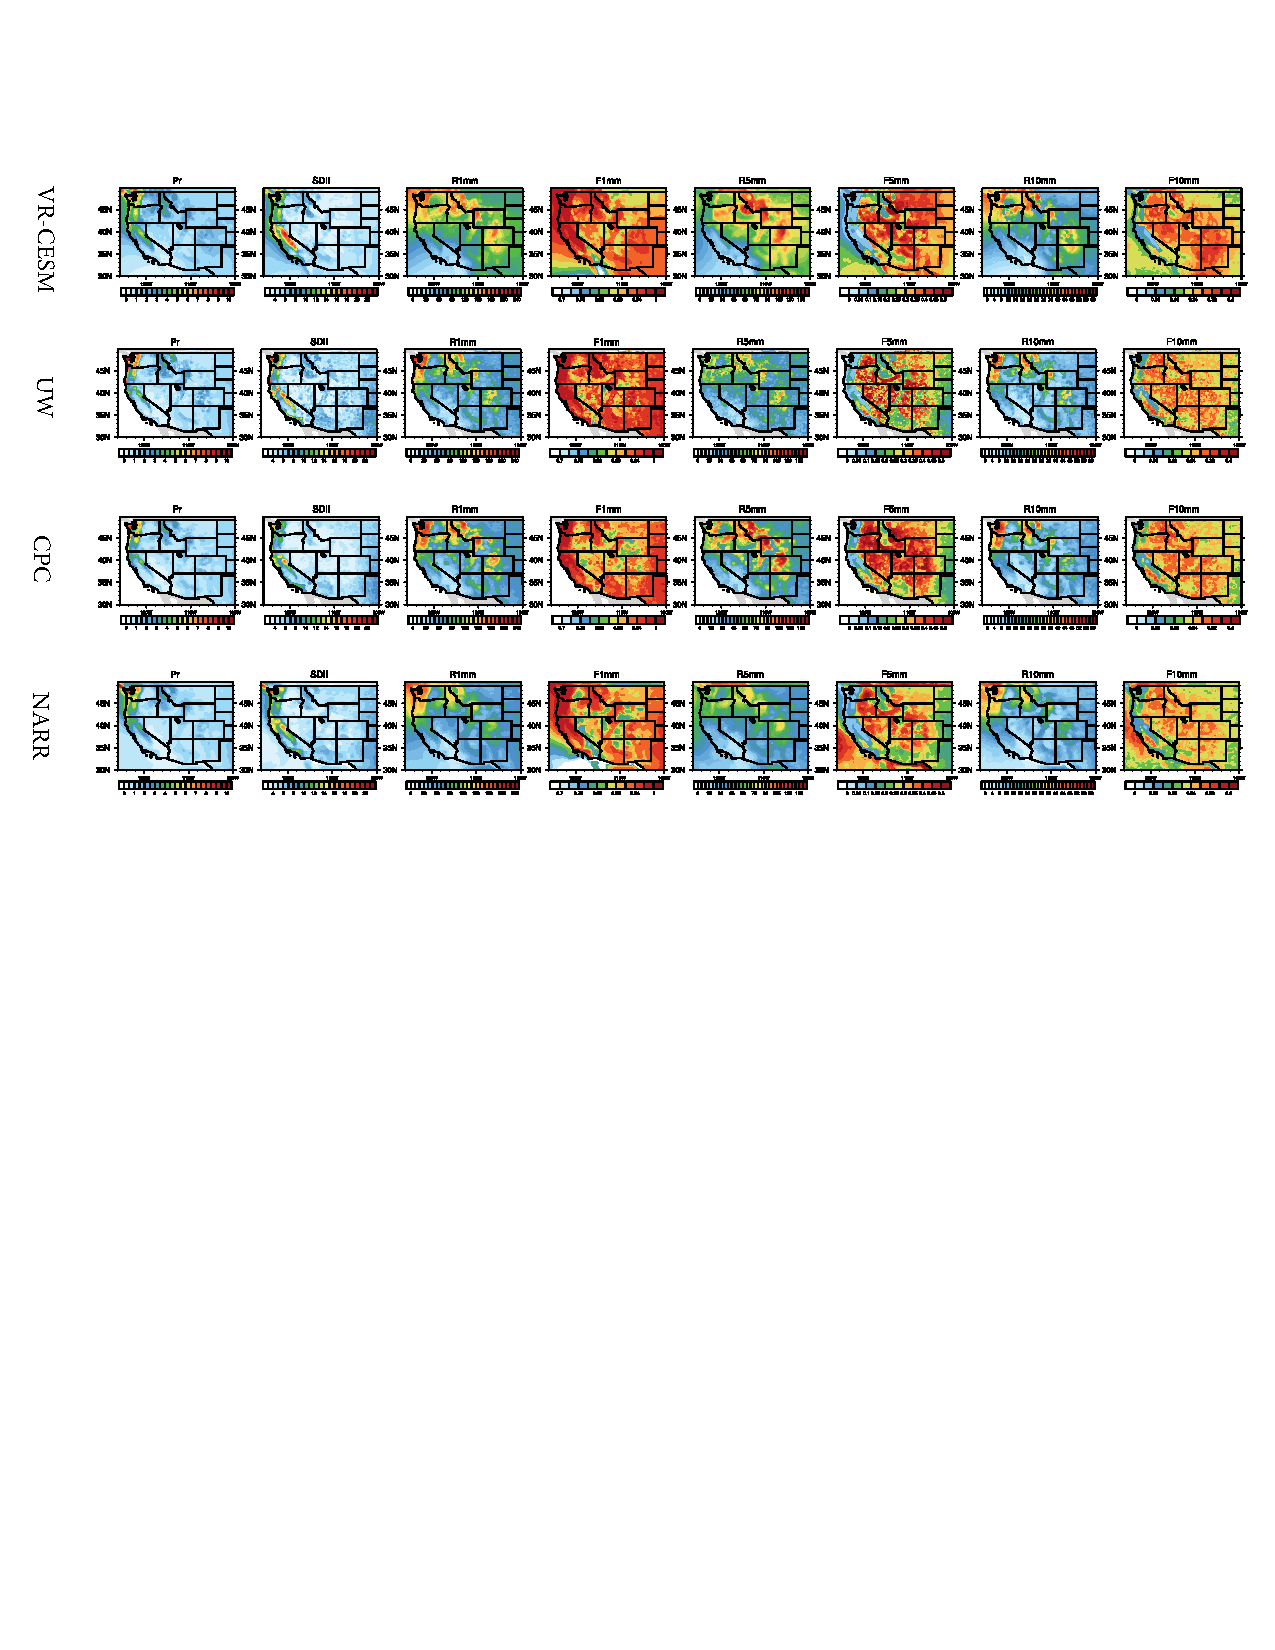
\includegraphics[width=6in]{wd_index_Hist_ref_annual_part1.pdf}
\caption{Mean precipitation and other related indices from VR-CESM and reference datasets over 1980-2005. (Note: Grids with statistically significance difference are marked with stippling.)}
\label{fig:histEval1}
\end{center}
\end{figure}

%Figure 3
\begin{figure}
\begin{center}
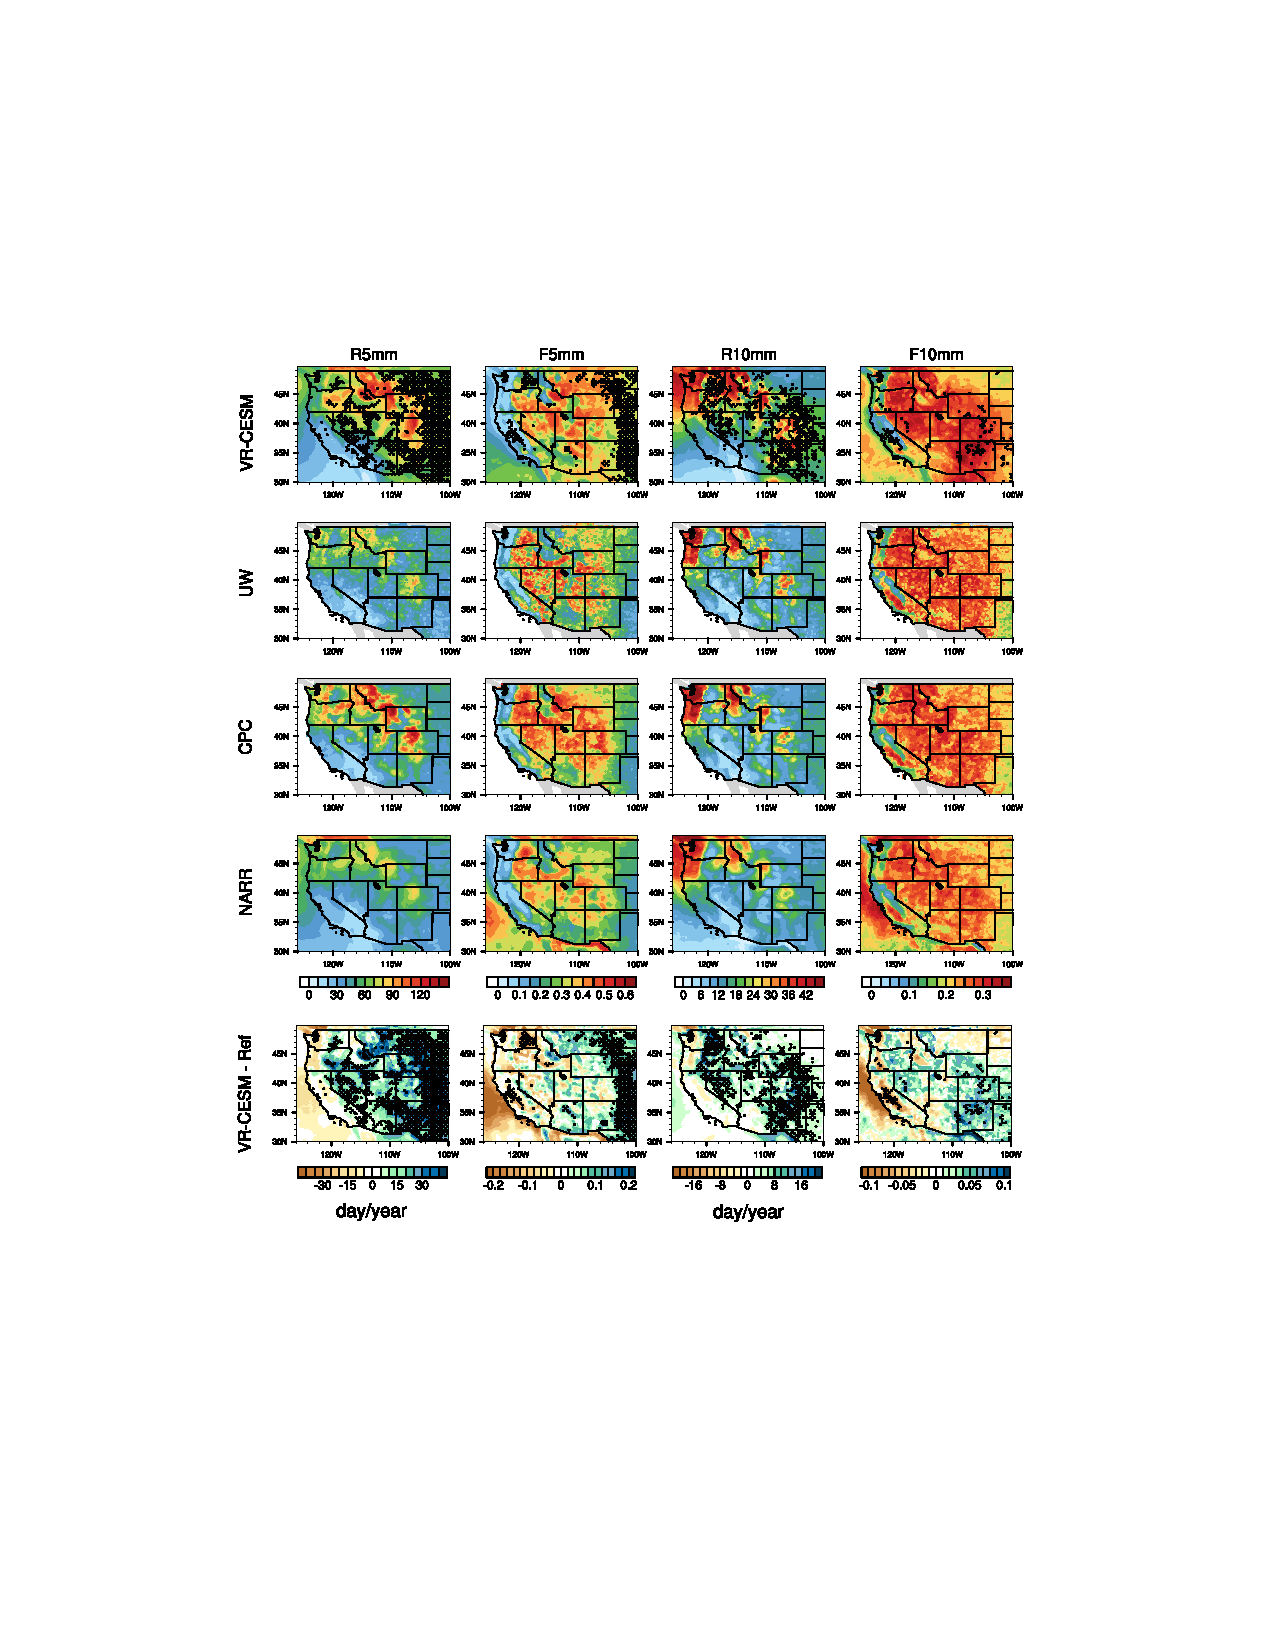
\includegraphics[width=6in]{wd_index_Hist_ref_annual_part2.pdf}
\caption{The mean precipitation and other related indices from VR-CESM and reference datasets over 1980-2005 (continued).}
\label{fig:histEval2}
\end{center}
\end{figure}

{\color{red}update the plot with new label levels}

%{\color{red}how about switch the row and column?}

%Figure 4
\begin{figure}
\begin{center}
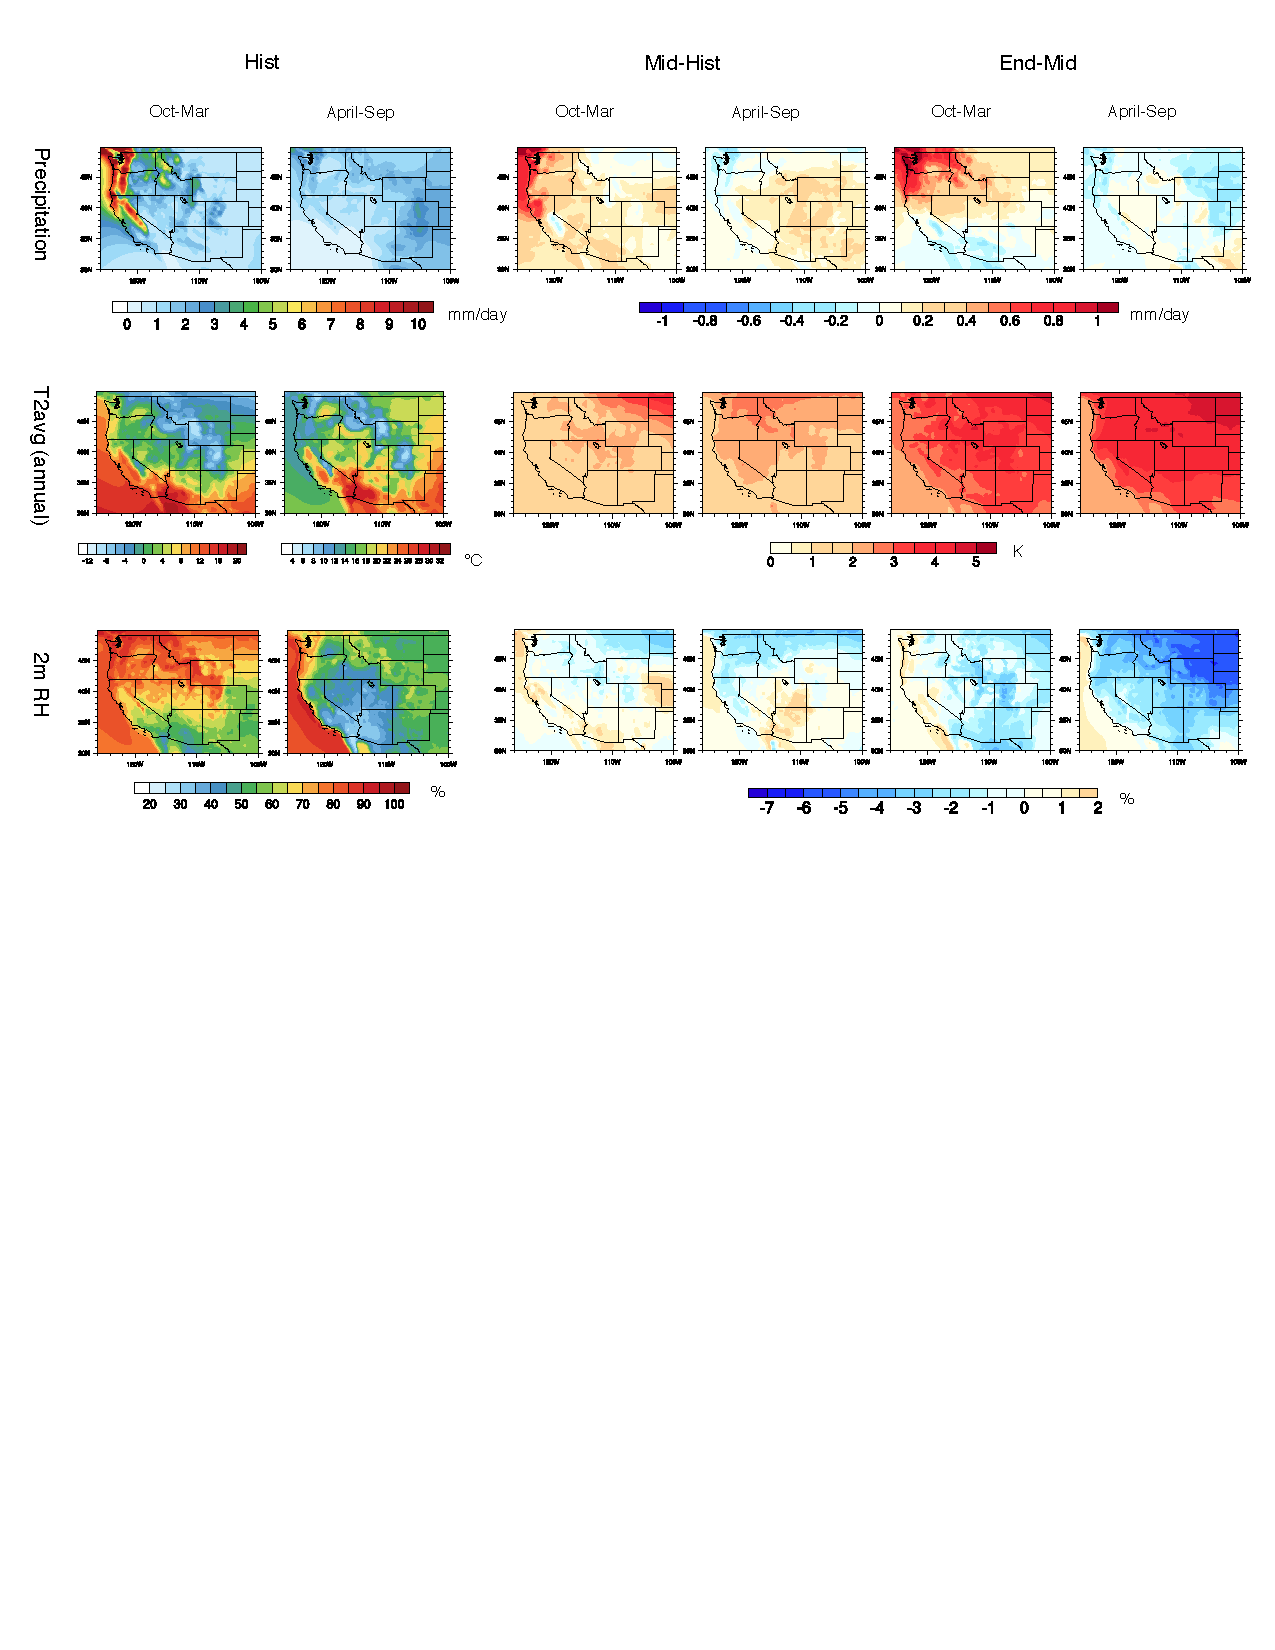
\includegraphics[width=6in]{pr_mean_clm.pdf}
\caption{The mean precipitation (Pr), 2m average temperature (T2avg), and 2m relative humidity (RH) averaged over each time period. (Note: Grids with statistically significance difference for the RH are marked with stippling.)}
\label{fig:meanClm}
\end{center}
\end{figure}

%Figure 5
\begin{figure}
\begin{center}
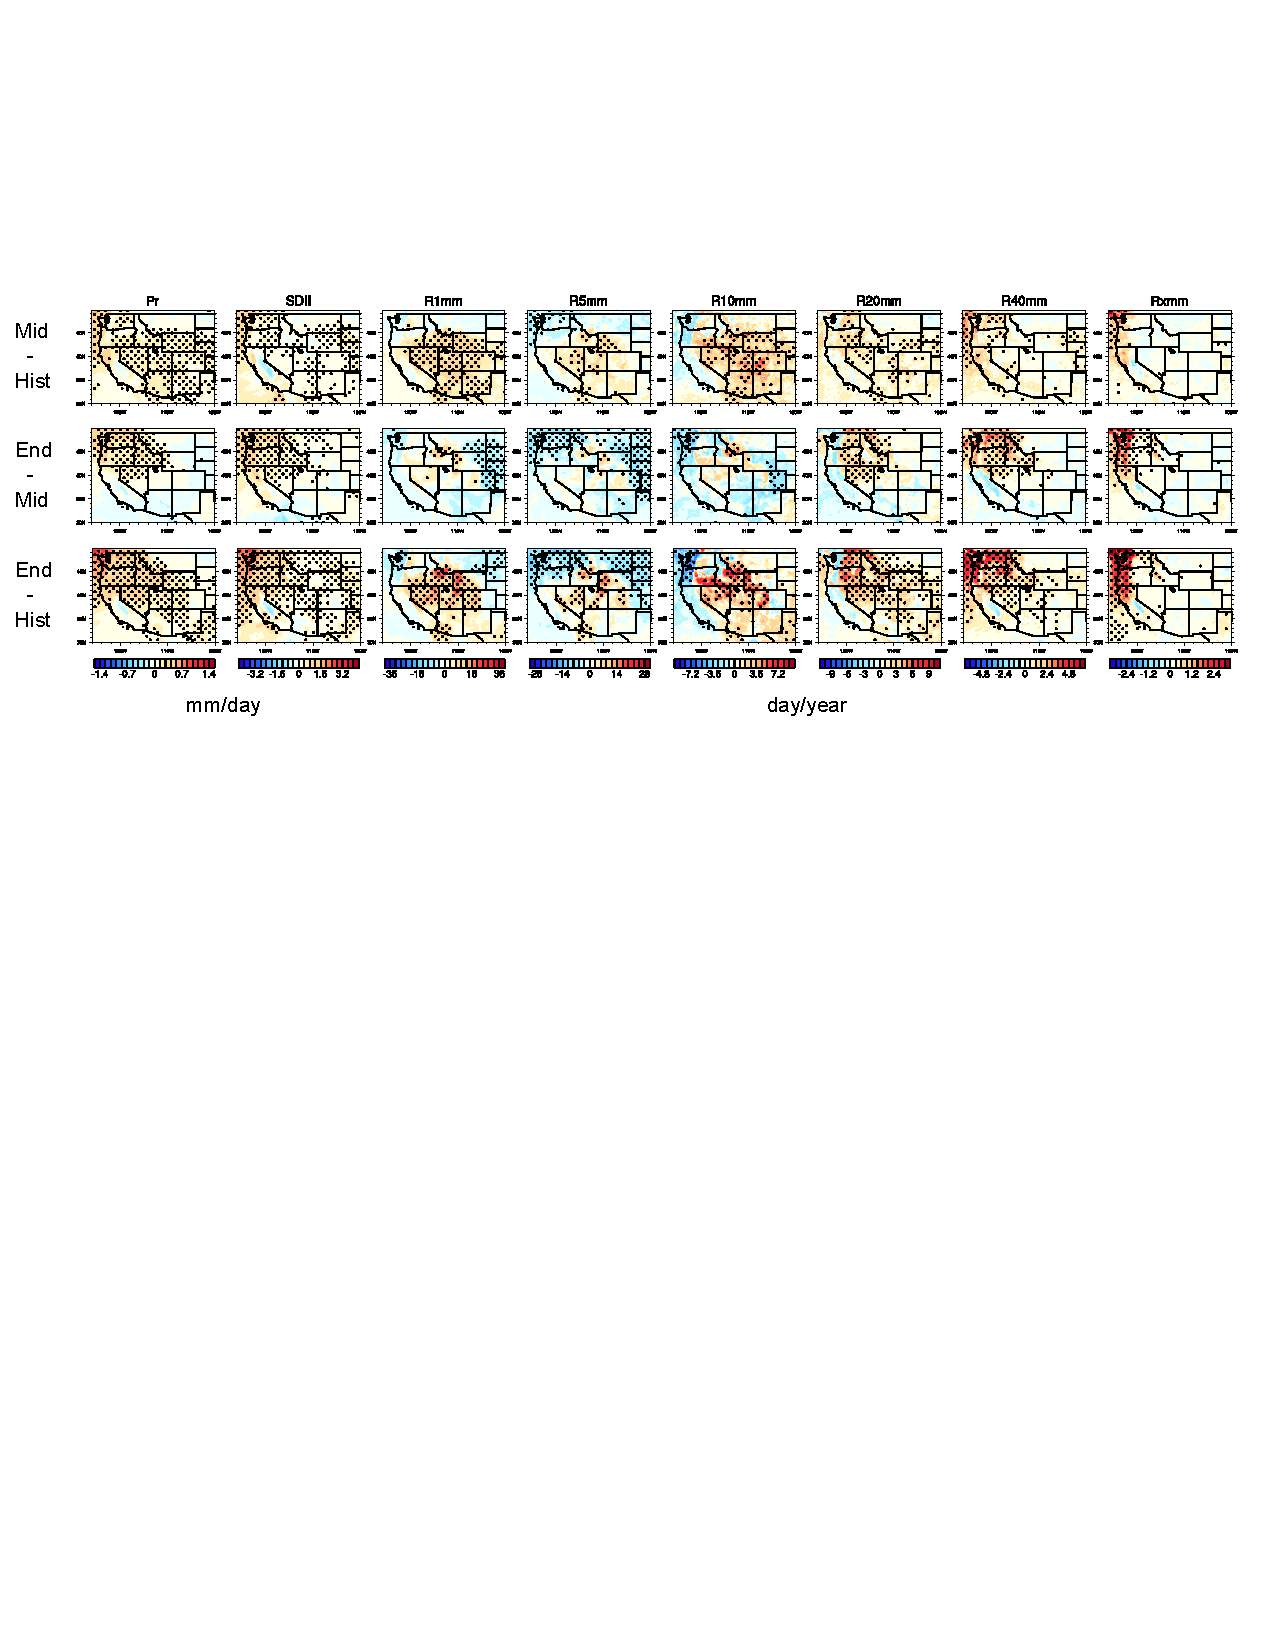
\includegraphics[width=6in]{wd_index_all_years_part1.pdf}
\caption{Differences of precipitation behaviors from past to future over WUS averaged of each time period. (Note: Grids with statistically significance difference are marked with stippling.) }
\label{fig:difIndex1}
\end{center}
\end{figure}

%(might add the mean intensity of each range), the mean intensity did not really change
%{\color{red}(might add the max1d and maxNd here.)}

%Figure 6
\begin{figure}
\begin{center}
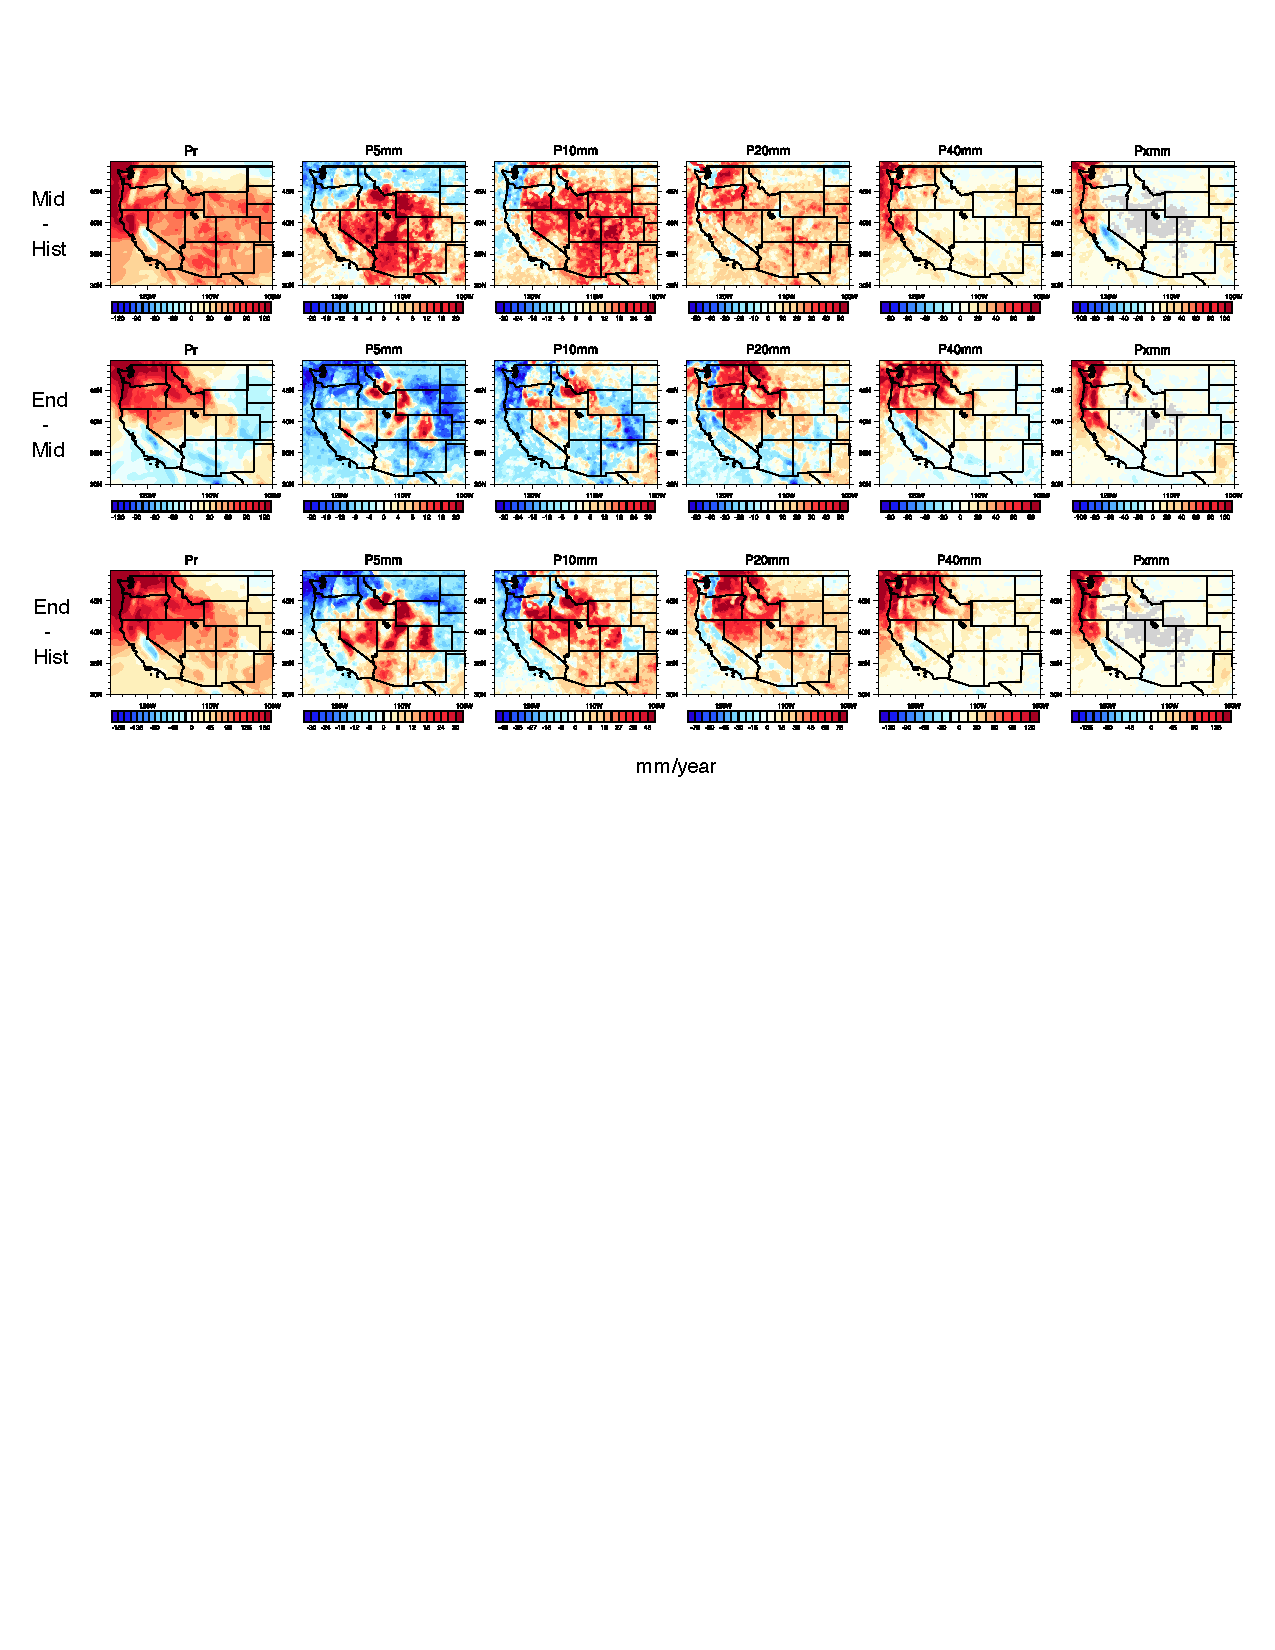
\includegraphics[width=6in]{wd_index_all_years_part2.pdf}
\caption{Differences of precipitation behaviors from past to future over WUS averaged of each time period (continued).}
\label{fig:difIndex2}
\end{center}
\end{figure}

%Figure 7
\begin{figure}
\begin{center}
\includegraphics[width=6in]{discussion_indices.pdf}
\caption{Changes of specific humidity and horizontal wind pattern at 850hPa for moisture flux illustration, and IVT for simulations under different time period of wet season (October to March). (Note: The minimum wind vector is set to be 0.5 m/s, therefore, the wind less than 0.5 m/s is also plotted at the minimum length for better visualization.) {\color{red}For all difference plots, make sure to use a common [min,max] range as its currently difficult to tease out differences.  Difference plots should also use a different color table to the mean results (perhaps a single color color table?). }}
\label{fig:discussIndex}
\end{center}
\end{figure}

%Figure 8
\begin{figure}
\begin{center}
\includegraphics[width=6in]{PP_PDF_region1_4.pdf}
\caption{Frequency distribution of rainy days (Pr$>=$0.1mm$/$day) over the three time periods from simulations in four regions (with logarithmic vertical scale). (Note: Region 1 to 4 cover Washington and Oregon; California; Nevada, Utah and Idaho; Arizona and New Mexico, respectively.)}
\label{fig:prPDF}
\end{center}
\end{figure}


%Figure 9
\begin{figure}
\begin{center}
\includegraphics[width=6in]{wd_index_enso_wetSeason.pdf}
\caption{Difference of precipitation behaviors between warm and cool phases of ENSO from past to future over WUS averaged of each time period.}
\label{fig:difEnso}
\end{center}
\end{figure}

%Figure 10
\begin{figure}
\begin{center}
\includegraphics[width=6in]{discussion_enso.pdf}
\caption{Changes of IVT for simulations under different phases of ENSO of wet season (October to March). (Note: The minimum wind vector is set to be 0.5 m/s, therefore, the wind less than 0.5 m/s is also plotted at the minimum length for better visualization.)}
\label{fig:discussEnso}
\end{center}
\end{figure}


\end{document}
